% !TEX TS-program = xelatex
% !TEX encoding = UTF-8
% !Mode:: "TeX:UTF-8"

\documentclass[onecolumn, oneside, ctexart]{SUSTechHomework}
\usepackage{float}
\usepackage{multicol}
\usepackage{cite}
\setlength{\parindent}{2em}
\linespread{1.5}
\lstset{language=sql}

\coursecode{CS307}
\coursename{Database Principle}
\title{Project 1}
\date{Oct. 1, 2021}

\begin{document}
  \maketitle
  \tableofcontents
  \pagebreak
  \setcounter{page}{1}

\section{结构设计}
\vspace{1em}
\centerline{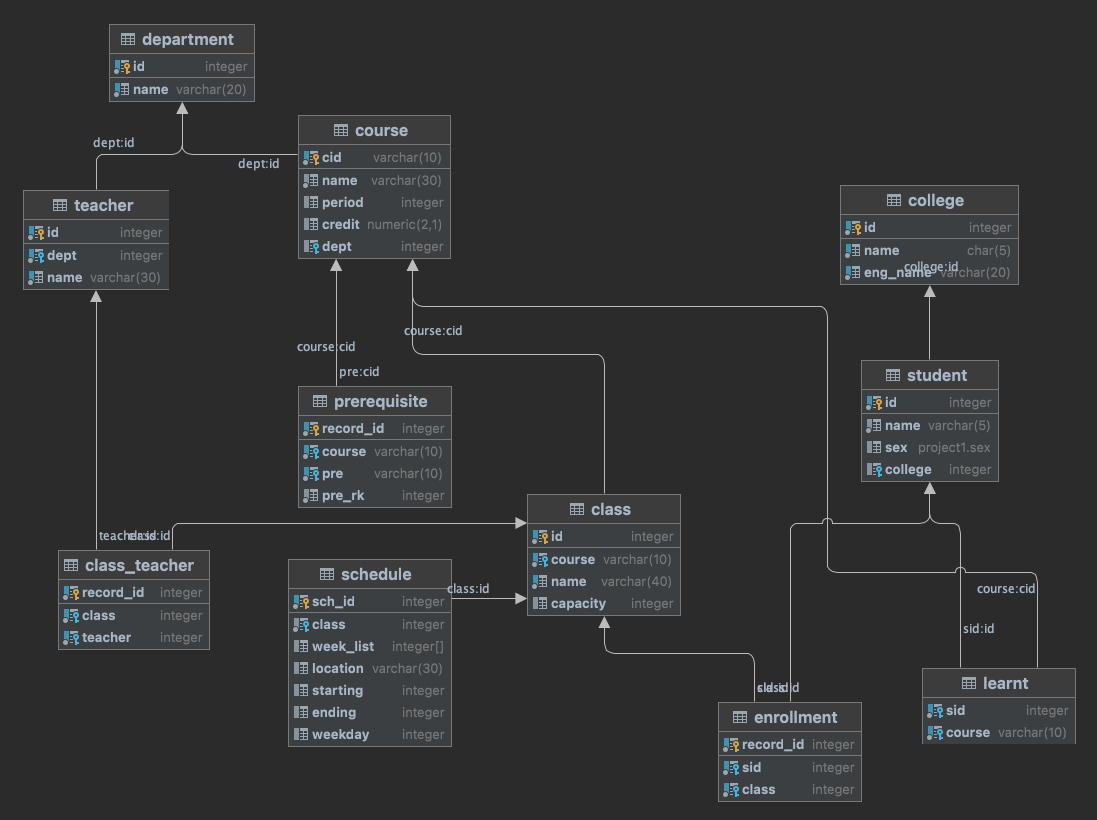
\includegraphics[width=0.9\textwidth]{./pic/ddl.png}}

\subsection{Department}
\begin{lstlisting}
CREATE TABLE department (
    id   serial PRIMARY KEY,
    name varchar(20) UNIQUE NOT NULL
);
\end{lstlisting}
\vspace{-3em}\par
无名的部门是无意义的,故为其加上非空约束,学校中的部门均不重名,即UNIQUE(name)。同时,此表有助于我们减少数据冗余、更方便进行部门更名或删除等操作,也允许了无成员的部门存在。
%Since there's no reason to store a department in each course's info (2NF) and teachers are belonged to departments, we store the information of departments in a table, we can easily add or change info by altering this table. Considering each department in a university surely has a unique name, and there's no reason to store a record with null name, there I put a UNIQUE NOT NULL constraint.

\subsection{Teacher}
\begin{lstlisting}
CREATE TABLE teacher (
    id   serial PRIMARY KEY,
    dept int         NOT NULL REFERENCES department (id),
    name varchar(30) NOT NULL,
    CONSTRAINT teacher_unk UNIQUE (dept, name)
);

\end{lstlisting}
\vspace{-3em}\par
%Each teacher belongs to a department, and it's possible that there exists several teachers in a university sharing the same name, but it's much less possible for it to happen in a single department, and we have no better way to recoginze this unless the data marks it, hence I assert the constraint \emph{name\_unk}.
考虑到学校中可能有重名的教师,而将范围缩小到一个院系里,出现重名的概率大大减少,在无明确指示的情况下我们可以认为部门一致、姓名一致即为同一个人。

\subsection{Course}
\begin{lstlisting}
CREATE TABLE course (
    cid    varchar(10) PRIMARY KEY,
    name   varchar(30) NOT NULL,
    period int CHECK (period > 0),
    credit numeric(2, 1) CHECK (credit >= 0),
    dept   int REFERENCES department (id)
);

\end{lstlisting}
\vspace{-3em}
\par
%This table stores courses like CS201 that may has multiple classes like Bilingual Class 1, 2 and 3. For these classes, they share the same syllabus thus we can aggregate course number \emph{cid}, course name, period, credit and dept into this level. For a course, its course number and name are critical and thus are not null, we can also check the validity of period and credit. Moreover, although there are differences between using int and varchar as primary key\textsuperscript{\cite{pk}}, considering the data volume, frequency of operations and complexity of query statements for later table calls, etc., I kept using course number as the primary key.
本项目共设计三个层次:\emph{course}(共享同一教学大纲)$\to$ \emph{class}(一门课程的多个教学班)$\to$ \emph{schedule}(某一教学班的上课安排)。与int型主键相比,使用varchar对后续的查询性能影响不大\textsuperscript{\cite{pk}},却更加方便查询,均衡二者考虑,选用课程号作为主键。并为\emph{period}(学时)及\emph{credit}(学分)加上合理的检查,减少数据库在经过多次数据更改后误操作修改为特别异常的可能性。

\subsection{Class}
\begin{lstlisting}
CREATE TABLE class (
    id       serial PRIMARY KEY,
    course   varchar(10) REFERENCES course (cid) NOT NULL,
    name     varchar(40)                         NOT NULL,
    capacity int CHECK (capacity > 0)
);
\end{lstlisting}
\vspace{-3em}\par
这里对课程容量进行检查,但允许其置空。另外,存在同一课程的多个班级同名的情况(FIN204有两个英文班),故不加UNIQUE约束。

\subsection{Class-Teacher}
\begin{lstlisting}
CREATE TABLE class_teacher (
    record_id serial PRIMARY KEY,
    class     int REFERENCES class (id)   NOT NULL,
    teacher   int REFERENCES teacher (id) NOT NULL,
    CONSTRAINT cls_tec_unk UNIQUE (class, teacher)
);
\end{lstlisting}
\vspace{-3em}\par
检查数据我们发现,部分班级缺失教师信息,但有教学班同时有数个教师。为了遵循第一范式,我们需要为某班级的所有教师均插入一条记录,且由实际情况可知这不会造成过度的数据膨胀。相比起在Class表中使用数组存教师,使用此表能更加方便的对教师安排进行调动,且能很方便的查询某门课的所有教师或某教师所教授的所有课程。

\subsection{Schedule}
\begin{lstlisting}
CREATE TABLE schedule (
    sch_id    serial PRIMARY KEY,
    class     int REFERENCES class (id) NOT NULL,
    week_list int[],
    location  varchar(30),
    starting  int CHECK (starting >= 1 AND starting <= 12),
    ending    int CHECK (ending >= 1 AND ending <= 12),
    weekday   int CHECK (weekday >= 1 AND weekday <= 7),
    CONSTRAINT time_valid CHECK (ending >= starting)
);
\end{lstlisting}
\vspace{-3em}\par
我们可以为课程时间进行细致的检查(如上四处CHECK所示),另外,考虑到周数列表往往平均长度超过10,若一昧追求1NF,表中将会存入超过教学班数目十倍的记录,且不便于删除,因此将其保存为数组,这样亦能很方便的检查、调整上课周数。

\subsection{Prerequisite}
\begin{lstlisting}
CREATE TABLE prerequisite (
    record_id serial PRIMARY KEY,
    course    varchar(10) REFERENCES course (cid) NOT NULL,
    pre       varchar(10) REFERENCES course (cid) NOT NULL,
    pre_rk    int                                 NOT NULL,
    CONSTRAINT preq_unk UNIQUE (course, pre)
);
\end{lstlisting}
\vspace{-3em}\par
课程的先修要求往往是$(A_1\lor \cdots A_n)\land \cdots \land (Z_1\lor\cdots\lor Z_n)$的形式,一般可将其先以“并且”分割为数块以“或者”链接的子关系。此时我们将“或块”分别标记为\emph{rank},每个rank中只需已学n一门课,且满足所有rank均学过即可。

\subsection{College}
\begin{lstlisting}
CREATE TABLE college (
    id       serial PRIMARY KEY,
    name     char(5) UNIQUE     NOT NULL,
    eng_name varchar(20) UNIQUE NOT NULL
);
\end{lstlisting}
\vspace{-3em}\par
存学生书院信息,这里将中英文名分别存放,并认为学校中所有书院的中、英文名均不相同。

\subsection{Student}
\begin{lstlisting}
CREATE TYPE sex AS enum ('M','F');

CREATE TABLE student (
    id      serial PRIMARY KEY,
    name    varchar(5) NOT NULL,
    sex     sex,
    college int REFERENCES college (id) DEFERRABLE
);
\end{lstlisting}
\vspace{-3em}\par
要保存一条学生记录应该至少知道学生姓名,故将name条目设为非空约束,而其余条目非关键信息可以为空;为了体现要求中"Use appropriate types for different fields of data"且"be as easy to expand as possible",选择用自定义枚举类保存性别,这相比起使用bool标识男女更加直观,且为将来新增性别增加了灵活性。

\subsection{Learnt}
\begin{lstlisting}
CREATE TABLE learnt (
    sid    int REFERENCES student (id) DEFERRABLE NOT NULL,
    course varchar(10) REFERENCES course (cid)    NOT NULL,
    CONSTRAINT learn_unk UNIQUE (sid, course)
);
\end{lstlisting}
\vspace{-3em}\par
数据中未给出选课具体教学班,从常理推测此应该为已学过课程。且学生-课程同时存在才作为一条有意义的记录,故两者均设为NOT NULL,另外认为修完一门课(无论是一次过还是挂科重修)均只留作一条记录,故加上UNIQUE。

\subsection{Enrollment}
\begin{lstlisting}
CREATE TABLE enrollment (
    record_id serial PRIMARY KEY,
    sid       int REFERENCES student (id) DEFERRABLE NOT NULL,
    class     int REFERENCES class (id)              NOT NULL,
    CONSTRAINT enroll_unk UNIQUE (sid, class)
);
\end{lstlisting}
\vspace{-3em}\par
此表存当前学期选课数据,即在开放选课时经过检查满足先修条件后允许插入,删除一条记录即为退课。在本次项目中此表留空。


\section{导入数据}
%\paragraph{Environment}
%\quad PostgreSQL 13.3\quad CentOS Linux release 7.9.2009 \quad Python 3.7.9\\

\subsection{数据清洗}
课程信息json文件的原始数据中包含大量空字符等无意义信息,也存在大量不遵循第一范式的条目。首先需要进行数据清洗,并将清洗完的数据存为新json文件,方便后面对比文件系统与数据库的性能时可以直接使用。而选课信息格式无需清洗,仅在插入数据库时需要检查是否重复以及有无对应课程。

\begin{lstlisting}[language=python]
import pandas as pd

def clear_data(ori: str, out: str):
    with open(ori) as f:
        cif = pd.read_json(f)

    nif = pd.DataFrame()
    nif['totalCapacity'] = cif['totalCapacity']
    nif['courseId'] = cif['courseId']
    nif['prerequisite'] = [clear_pre(pre) for pre in cif['prerequisite']]
    nif['courseHour'] = cif['courseHour']
    nif['courseCredit'] = cif['courseCredit']
    nif['courseName'] = [clear_str(c) for c in cif['courseName']]
    nif['className'] = [clear_str(c) for c in cif['className']]
    nif['courseDept'] = cif['courseDept']
    nif['teacher'] = [clear_teacher(t) for t in cif['teacher']]
    nif['classList'] = clear_class_list(cif['classList'])

    with open(out, 'w+', encoding='utf-8') as f:
        f.write(nif.to_json(orient='records', force_ascii=False))
\end{lstlisting}

\vspace{-3em}\par
我们使用Pandas来更灵活的管理数据框架,检查数据后发现需要清洗的数据为以下几类:
\paragraph{courseName}首位存在空字符,且全半角使用不统一。我们将数据统一使用半角符号,查询时也将用户输入的查询条件清洗为半角即可。
\begin{lstlisting}[language=python]
def clear_str(s):
    if s is None:
        return None
    return s.strip() \
        .replace('(', '(') \
        .replace(')', ')') \
        .replace(',', ',')
\end{lstlisting}
\vspace{-3em}
\begin{lstlisting}[language=python]
>>> clear_str('文物精品研究鉴赏  ')
    '文物精品研究鉴赏'
>>> clear_str('高等数学(下)A')
    '高等数学(下)A'
\end{lstlisting}
\vspace{-3em}

\paragraph{teacher}教师列表不仅存在空字符,也不满足第一范式,我们直接将其处理为Python列表。
\begin{lstlisting}[language=python]
def clear_teacher(t):
    if t is None:
        return None
    return [t.strip() for t in clear_str(t).split(',')]
\end{lstlisting}
\vspace{-3em}
\begin{lstlisting}[language=python]
>>> clear_teacher('\t唐珂 ,  汤小菊\n , Alan Turing  , 于仕琪 '))
	['唐珂', '汤小菊', 'Alan Turing', '于仕琪']
\end{lstlisting}
\vspace{-3em}

\paragraph{prerequisite}
首先按“与”关系分割为数个“或”关系簇,再将其分割为单个课程。有些课程存在多种形式,并存在重复的多项,但为了体现DBMS的性能,这里不做处理,由DBMS负责。其难点在于需要清楚逻辑关系的括号,而不能影响到课程名中的括号,否则课程名中带括号或原有括号被删将影响数据库对课程号的匹配。
\begin{lstlisting}[language=python]
def clear_pre(pre):
    if pre is None:
        return None
    return [[ors.strip('() ') + (')' if ors.strip('() ').endswith(('上', '下')) else '')
             for ors in ands.split('或者')]
            for ands in pre.split('并且')]
\end{lstlisting}
\vspace{-3em}
\begin{lstlisting}[language=python]
>>> clear_pre('(高等数学(下)A 或者 高等数学(下) 或者 数学分析II) 并且 (大学物理A(下) 或者 大学物理 B(下) 或者 大学物理A(下)) 并且 (线性代数I-A 或者 线性代数I)')
    [['高等数学(下)A', '高等数学(下)', '数学分析II'], ['大学物理A(下)', '大学物理 B(下)', '大学物理A(下)'], ['线性代数I-A', '线性代数I']]
\end{lstlisting}
\vspace{-3em}

\paragraph{classList}
其内部又分为多个可能需要清洗的项:
\begin{lstlisting}[language=python]
def clear_class_list(df):
    class_list = []
    for cls in df:
        cls_items = []
        for item in cls:
            item_cls = {}
            item_cls.update({'weekList': [int(x) for x in item.get('weekList')]})
            item_cls.update({'location': clear_str(item.get('location'))})
            item_cls.update({'classTime': item.get('classTime')})
            item_cls.update({'weekday': item.get('weekday')})
            cls_items.append(item_cls)
        class_list.append(cls_items)
    return class_list
\end{lstlisting}
\vspace{-1em}
\centerline{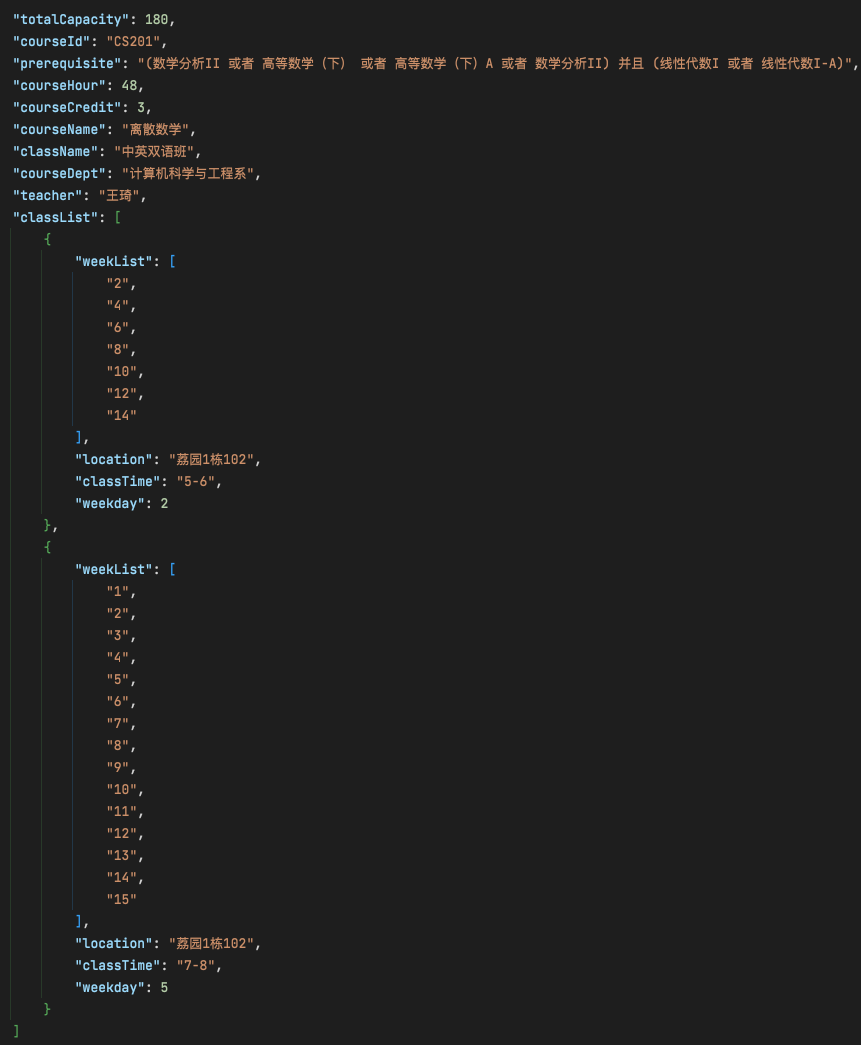
\includegraphics[height=7cm]{dta/clbf.png}\qquad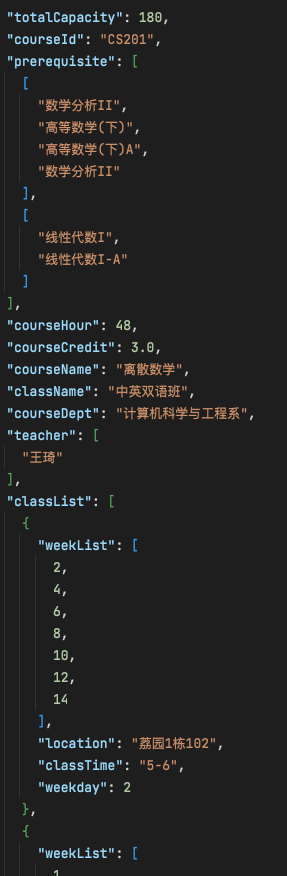
\includegraphics[height=7cm]{dta/claf.png}}
\scriptsize
\centerline{数据清洗前后对比}
\normalsize

\subsection{导入课程信息}
本部分数据量远小于选课数据,因此我们注重于导入的准确性(优化速度的方案于下节展开讨论)。
\par 由于此部分外键限制错综复杂,若只导一次数据,各种子查询及外键冲突处理等会使得DML变得异常复杂且可读性较低,因此,以下我们多次遍历数据,将存在外键约束的条目分别开来。
\begin{lstlisting}[language=python]
import psycopg2 as psql
from psycopg2.extras import execute_batch
# import other packages

class DB:
    def __init__(self, conf: str = './user.yml', data='./data/clear_course_info.json'):
        with open(conf, 'r', encoding='utf-8') as cfg:
            conf = yaml.safe_load(cfg)
        try:
            self.conn = psql.connect(host=conf['host'], port=conf['port'],
                                     user=conf['user'], password=conf['pwd'],
                                     database=conf['db'])
            self.cur = self.conn.cursor()
            self.conn.autocommit = False
        except Exception as e:
            print(e)
            sys.exit(1)
        with open(data, 'r') as dat:
            self.cdata = pd.read_json(dat)
        print('Database connected && Data loaded to RAM.')

    def __del__(self):
        self.conn.commit()
        self.conn.close()
\end{lstlisting}
\vspace{-3em}\par
这里定义了DB类,并在实例化对象时自动连接数据库(连接所需密码、数据库等信息由配置文件读取而得)并将数据载入内存;程序结束销毁对象时进行一次提交并关闭链接。

\begin{lstlisting}[language=python]
def submitter(self, time_start, sql, data):
    print(f'Preparing data in py ({time.perf_counter() - time_start:.4f}s)', end=' >>> ')
    try:
        tm = time.perf_counter()
        execute_batch(self.cur, sql, data)
        self.conn.commit()
        print(f'Submitted {len(data)} requests '
              f'({time.perf_counter() - tm:.4f}s | avg={len(data) / (time.perf_counter() - tm):.4f}i/s)')
    except Exception as e:
        print(e)
\end{lstlisting}
\vspace{-3em}\par
通用提交插入命令的函数,完成了计时,使用批处理(细节于下节讨论)。

\begin{lstlisting}[language=python]
def create_tables(self, ddl_path):
    with open(ddl_path, 'r') as dl:
        sql_list = dl.read().split(';')[:-1]
    try:

        for sql_item in sql_list:
            self.cur.execute(sql_item)
        self.conn.commit()
    except Exception as e:
        print(repr(e))
\end{lstlisting}
\vspace{-3em}\par
为了实现高度的自动化,这里将第一节的DDL及以下两句命令写入SQL文件中。利用PostgreSQL命令由分号结束的性质,此函数逐句执行SQL文件中的命令(删除原有schema并重新建表)。

\begin{lstlisting}
DROP SCHEMA IF EXISTS project1 CASCADE;
CREATE SCHEMA project1;
\end{lstlisting}

\begin{lstlisting}[language=python]
@timer
def ins_dept(self):
    sql = '''
            INSERT INTO project1.department (name)
            VALUES (%s)
            ON CONFLICT DO NOTHING;
          '''
    tm = time.perf_counter()
    dept = [(x,) for x in self.cdata['courseDept']]
    self.submitter(tm, sql, dept)

@timer
def ins_teacher(self):
    sql = '''
            INSERT INTO project1.teacher(name, dept)
            VALUES (%s, (SELECT id
                         FROM project1.department
                         WHERE name = %s))
            ON CONFLICT DO NOTHING;
          '''
    tm = time.perf_counter()
    teacher = []
    for index, item in self.cdata.iterrows():
        if item['teacher'] is None:
            continue
        for t in item['teacher']:
            teacher.append((t, item['courseDept']))
    self.submitter(tm, sql, teacher)

@timer
def ins_course(self):
    sql = '''
            INSERT INTO project1.course
            VALUES (%s, %s, %s, %s, (SELECT id
                                     FROM project1.department
                                     WHERE name = %s))
            ON CONFLICT DO NOTHING;
          '''
    tm = time.perf_counter()
    course = [(item['courseId'], item['courseName'], item['courseHour'],
               item['courseCredit'], item['courseDept'])
              for index, item in self.cdata.iterrows()]
    self.submitter(tm, sql, course)

@timer
def ins_pre(self):
    sql = '''
            WITH preid AS (SELECT cid
                           FROM project1.course
                           WHERE name = %s)
            INSERT INTO project1.prerequisite (course, pre, pre_rk)
                (SELECT %s, (SELECT cid FROM preid LIMIT 1), %s
                 WHERE (SELECT COUNT(cid) FROM preid) > 0)
            ON CONFLICT DO NOTHING;
          '''
    tm = time.perf_counter()
    pres = []
    for index, item in self.cdata.iterrows():
        if item['prerequisite'] is None:
            continue
        for rk, ands in enumerate(item['prerequisite'], start=1):
            for ors in ands:
                pres.append((ors, item['courseId'], rk))
    self.submitter(tm, sql, pres)
\end{lstlisting}
\vspace{-3em}\par
实现避免插入重复一般有两种方案:\ding{172} INSERT INTO <table> (SELECT <values> WHERE (SELECT COUNT(*) FROM <table>) = 0,可见该方法不仅书写复杂,本地为了填充批处理命令也需要准备更多数据;\ding{173} INSERT INTO <table> VALUES (<values>) ON CONFLICT DO NOTHING,不仅书写简单,填充数据少,且DBMS计划任务较简单,执行更快。\\~\\
\centerline{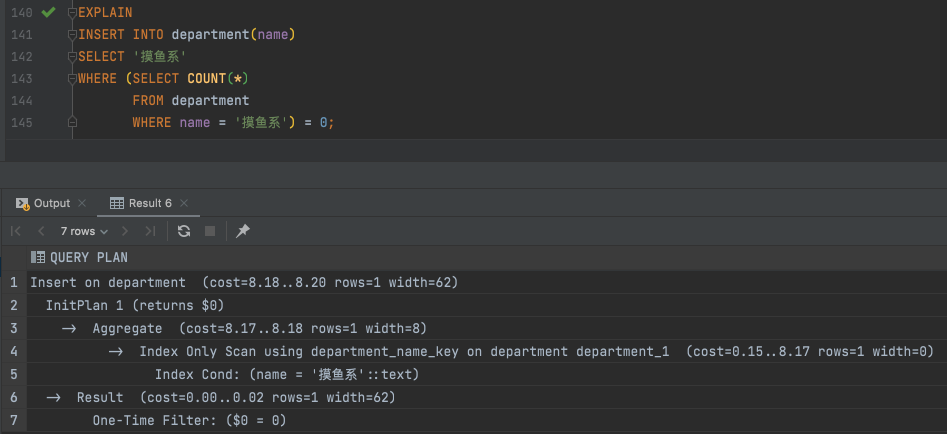
\includegraphics[height=4cm]{dta/ins1.png}\qquad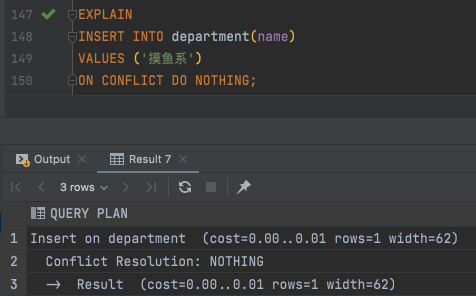
\includegraphics[height=4cm]{dta/ins2.png}}
~\\
\centerline{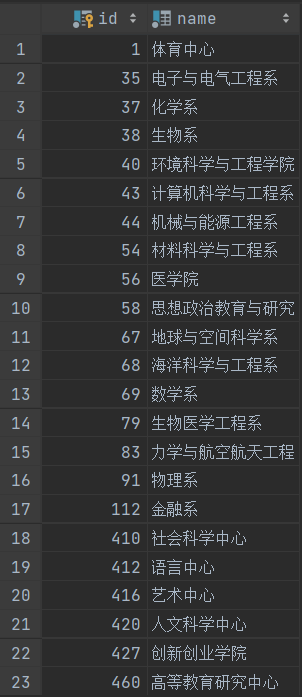
\includegraphics[height=4.5cm]{dta/dept.png}
\quad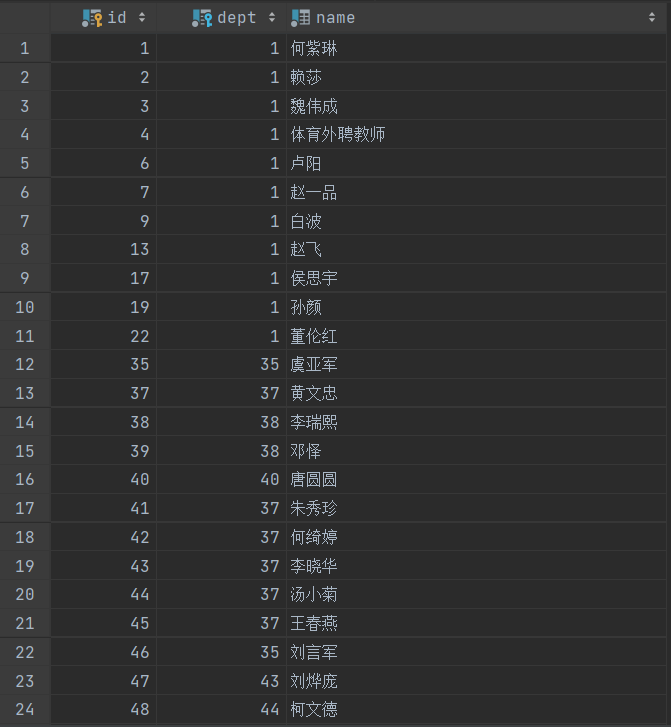
\includegraphics[height=4.5cm]{dta/tech.png}
\quad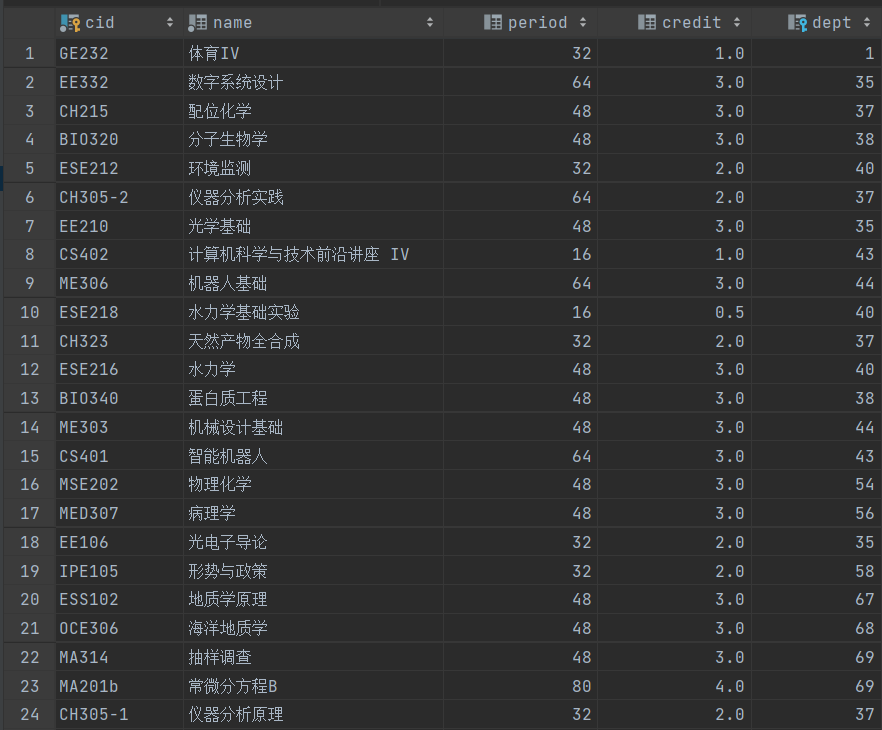
\includegraphics[height=4.5cm]{dta/course.png}
\quad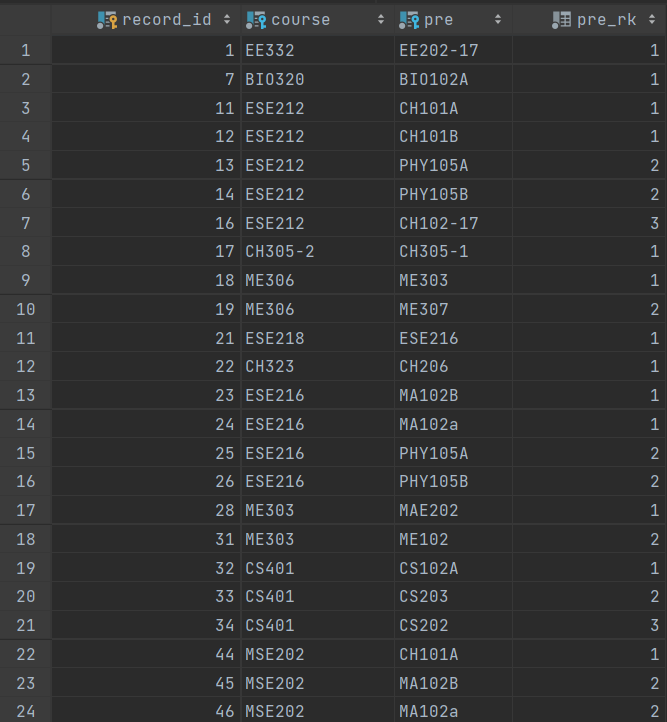
\includegraphics[height=4.5cm]{dta/preq.png}}
\scriptsize\centerline{上示正确插入后的数据存储}\normalsize
~\\

\begin{lstlisting}[language=python]
@timer
def ins_class_te_sc(self):
        sql_cls = '''
                    INSERT INTO project1.class
                    VALUES (%s, %s, %s, %s);
                  '''
        sql_tec = '''
                    WITH tid AS (
                    SELECT id
                    FROM project1.teacher
                    WHERE name = %s
                        AND dept = (SELECT id FROM project1.department WHERE name = %s)
                    )
                    INSERT INTO project1.class_teacher (class, teacher)
                    VALUES (%s, (SELECT id FROM tid));
                  '''
        sql_sch = '''
                    INSERT INTO project1.schedule (class, week_list, location, starting, ending, weekday)
                    VALUES (%s, %s::int[], %s, %s, %s, %s);
                  '''
        tm = time.perf_counter()
        cls = []
        tec = []
        sch = []
        self.cur.execute('''
                           SELECT GREATEST((SELECT last_value - 1
                                            FROM project1.class_id_seq),
                                           (SELECT MAX(id)
                                            FROM project1.class));
                         ''')
        for idx, (index, item) in enumerate(self.cdata.iterrows(), start=self.cur.fetchone()[0] + 1):
            cls.append((idx, item['courseId'], item['className'], item['totalCapacity']))
            if item['teacher'] is not None:
                for x in iter((t, item['courseDept'], idx) for t in item['teacher']):
                    tec.append(x)
            for x in iter((idx,
                           str(cl.get('weekList')).replace('[', '{').replace(']', '}'),
                           cl.get('location'),
                           int(cl.get('classTime').split('-')[0]),
                           int(cl.get('classTime').split('-')[1]),
                           cl.get('weekday'))
                          for cl in item['classList']):
                sch.append(x)
        print(f'Preparing data in py ({time.perf_counter() - tm:.4f}s)', end=' >>> ')
        try:
            tm = time.perf_counter()
            execute_batch(self.cur, sql_cls, cls)
            execute_batch(self.cur, sql_tec, tec)
            execute_batch(self.cur, sql_sch, sch)
            self.cur.execute('SELECT max(id) FROM project1.class')
            self.cur.execute('ALTER SEQUENCE project1.class_id_seq RESTART WITH %s;',
                             self.cur.fetchone()[0] + 1)
            self.conn.commit()
            print(f'Submitted {len(cls) + len(tec) + len(sch)} requests '
                  f'({time.perf_counter() - tm:.4f}s | '
                  f'avg={(len(cls) + len(tec) + len(sch)) / (time.perf_counter() - tm):.4f}i/s)')
        except Exception as e:
            print(e)
\end{lstlisting}
\vspace{-3em}\par
这里我们同时向Class,Class-Teacher和Schedule插入字段。常规的做法是先插入Class,以后在插入Class-Teacher的cid等字段时进行大量的SELECT id操作,显然这非常耗时。考虑到json文件中按教学班存信息,我们可以管理本地index,使得每个Class的index互异且递增(如31行所示),并将相同的index填入此教学班所属的时段和教师。
\par 为了避免主键的UNIQE冲突,我们首先要检测当前表中最大自增ID号及实际存的最大index(在本例中我们知道本地index从1开始即可,但此检测提高了程序的鲁棒性,避免了向非空的表中插入数据时产生的index冲突),并在插入数据后重设DBMS的自增序列(如51行所示),这保证了在以后的插入中如果不指定index,使用自增id不会导致异常。\\~\\
\centerline{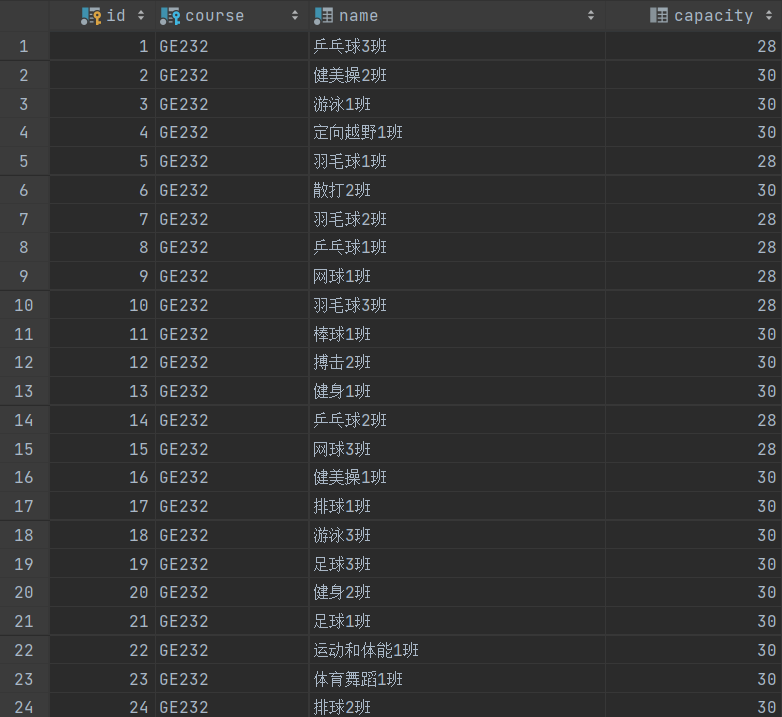
\includegraphics[height=4.2cm]{dta/class.png}\quad
	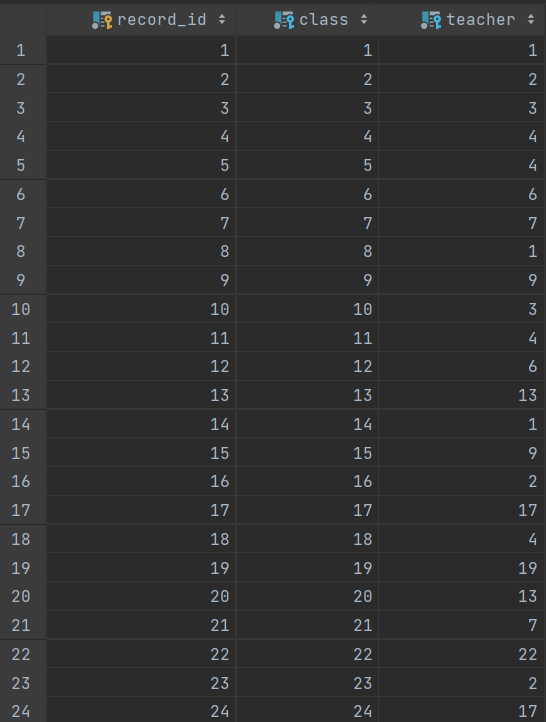
\includegraphics[height=4.2cm]{dta/ct.png}\quad
	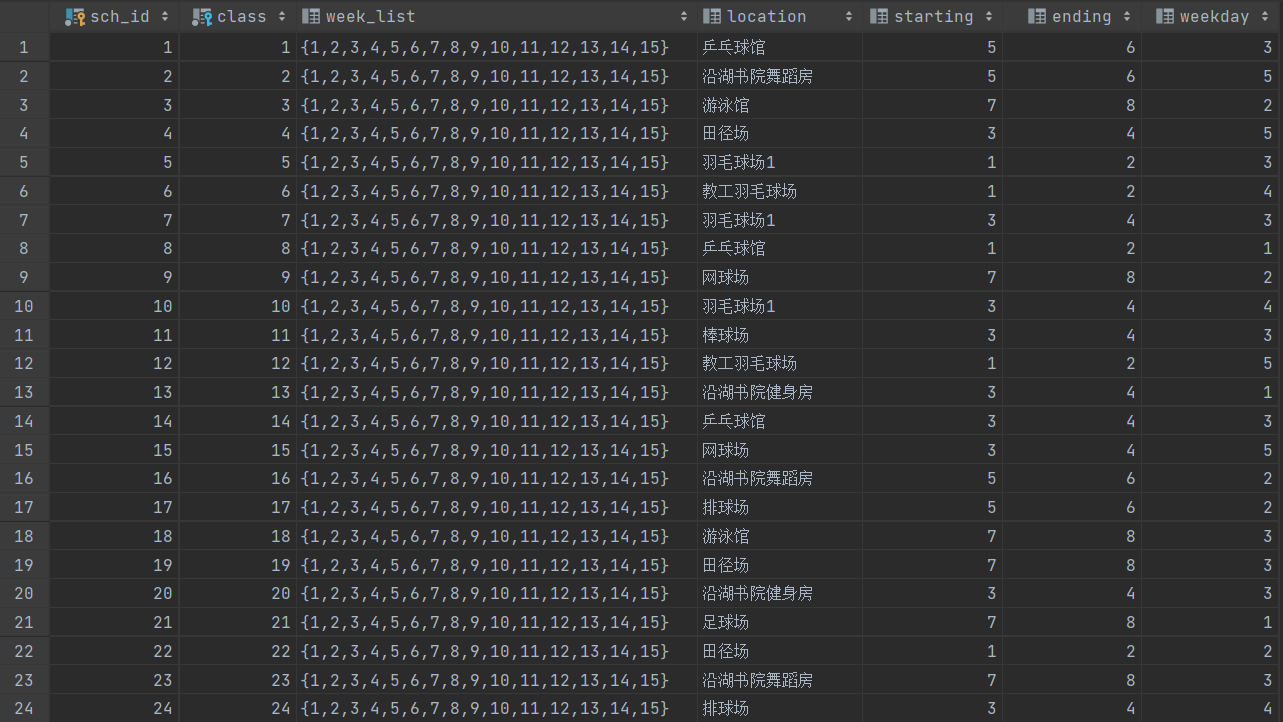
\includegraphics[height=4.2cm]{dta/sch.png}}\\~\\
\centerline{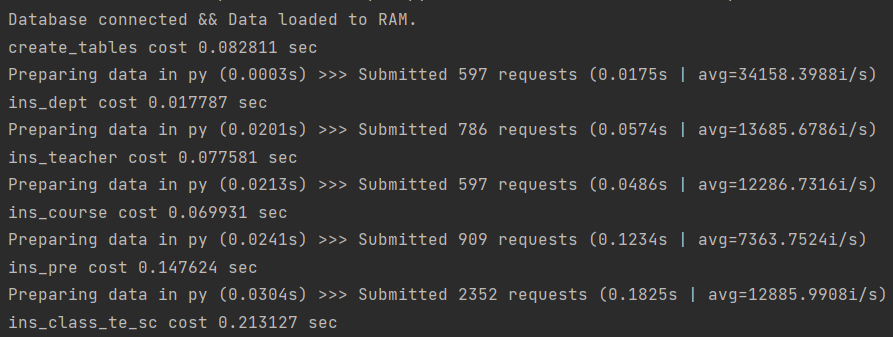
\includegraphics[height=3.5cm]{dta/cisp.png}}
\scriptsize\centerline{插入课程信息平均速度16075 items/sec}\normalsize

\subsection{导入选课信息}
\subsubsection{关闭自动提交}
\begin{lstlisting}[language=python]
@timer
def bad_loader(self):
    for stu in self.cdata:
        try:
            self.cur.execute('''INSERT INTO project1.college(name, eng_name)
                                SELECT %s, %s
                                WHERE (SELECT COUNT(*)
                                       FROM project1.college
                                       WHERE name = %s) = 0;''',
                             (stu[2].split('(')[0],
                              stu[2].split('(')[1].replace(')', ''),
                              stu[2].split('(')[0]))
            self.cur.execute('''INSERT INTO project1.student
                                VALUES (%s, %s, %s, (SELECT id
                                                     FROM project1.college
                                                     WHERE name = %s))
                                ON CONFLICT DO NOTHING;''',
                             (stu[3], stu[0], stu[1], stu[2].split('(')[0]))
            for sel in stu[4:]:
                self.cur.execute('''INSERT INTO project1.learnt
                                    (SELECT %s, %s
                                     WHERE EXISTS(SELECT id FROM project1.student WHERE id = %s)
                                       AND EXISTS(SELECT cid FROM project1.course WHERE cid = %s))
                                     ON CONFLICT DO NOTHING;''',
                                 (stu[3], sel, stu[3], sel))
        except Exception as e:
            print(e)
\end{lstlisting}
\vspace{-3em}\par
需要注意的是psycopg2在建立连接后默认关闭自动提交。实验对比可知相比于autocommit时的插入速度,关闭其将性能提升了约36.7\%。
~\\
\begin{figure*}[!h]
	\centering
	\begin{subfigure}[b]{0.8\textwidth}
		\centerline{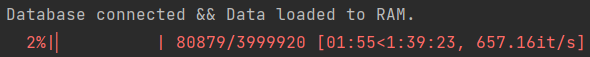
\includegraphics[width=0.6\textwidth]{./sp/autocommit.png}}
		\caption{autocommit = true}
	\end{subfigure}\\
	\begin{subfigure}[b]{0.8\textwidth}
		\centerline{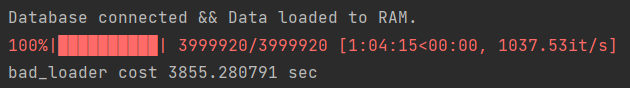
\includegraphics[width=0.6\textwidth]{./sp/bl.png}}
		\caption{autocommit = false, bad\_loader}
	\end{subfigure}	
	\label{fig:visual_smap}
\end{figure*}
\par 分析其原因,自动提交时需要频繁检查数据是否满足ACID,越早插入的数据受越多次检查,从而耗费大量时间;而关闭自动提交大大减少了检测的次数以及每行被检测的平均次数。

\subsubsection{批处理及分页大小}
\begin{lstlisting}[language=python]
@timer
def batch_loader(self, pg: int):
    # prepare data
    try:
        execute_batch(self.cur,
                      '''INSERT INTO project1.college(name, eng_name)
                         SELECT %s, %s
                         ON CONFLICT DO NOTHING;''',
                      college,
                      page_size=pg)
        # similar for student info and course selection
    except Exception as e:
        print(e)
\end{lstlisting}
\vspace{-3em}\par
使用批处理 (psycopg2.extras.execute\_batch) 使得一次操作中可以执行多条SQL语句,相比于一次一次执行效率会提高很多。理论上在一定范围内,batch size (page\_size) 越大,批量操作需要向数据库发送请求的次数越少,速度就越快;以下实验测得当分页大小为1000左右时相较于较小的分页大小有较好的提速效果,但当其进一步加大时(下图(d)),速度反而下降,相较于减少请求次数带来的时间损耗,单次发送请求过大反而降低效果。本项可最多带来约21.7\%的性能提升。
~\\
\begin{figure*}[!h]
	\centering
	\begin{subfigure}[b]{0.8\textwidth}
		\centerline{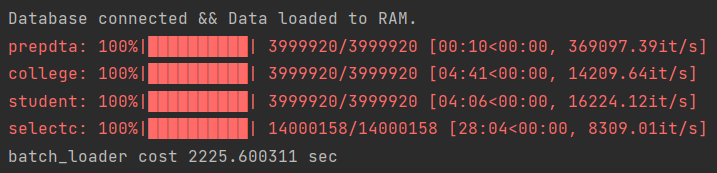
\includegraphics[width=0.6\textwidth]{./sp/batch100.png}}
		\caption{batch size = 100}
	\end{subfigure}\\
	\begin{subfigure}[b]{0.8\textwidth}
		\centerline{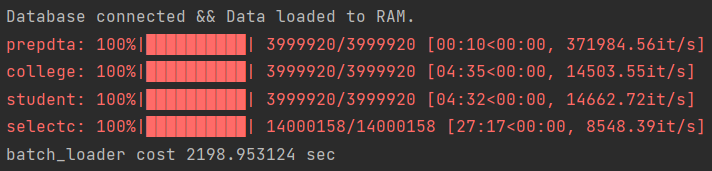
\includegraphics[width=0.6\textwidth]{./sp/batch500.png}}
		\caption{batch size = 500}
	\end{subfigure}	
	\begin{subfigure}[b]{0.8\textwidth}
		\centerline{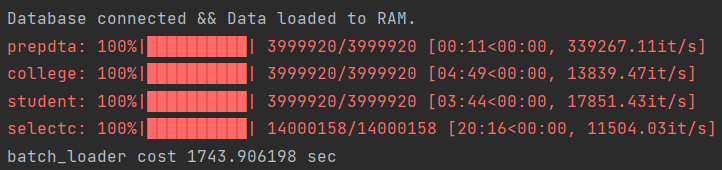
\includegraphics[width=0.6\textwidth]{./sp/batch1000.png}}
		\caption{batch size = 1000}
	\end{subfigure}\\
	\begin{subfigure}[b]{0.8\textwidth}
		\centerline{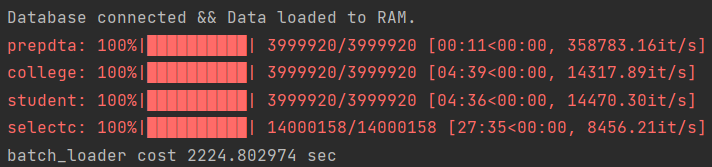
\includegraphics[width=0.6\textwidth]{./sp/batch1500.png}}
		\caption{batch size = 1500}
	\end{subfigure}	
	\label{fig:visual_smap}
\end{figure*}

\subsubsection{延迟检查外键约束}
呼应前面建表中的\emph{deferrable},只需要在batch的基础上加上以下两句就可以在插入事务块中暂时不检查外键约束,而在插入完成后统一检查。
\begin{lstlisting}[language=python]
self.cur.execute('BEGIN TRANSACTION;')
self.cur.execute('SET CONSTRAINTS ALL DEFERRED;')
\end{lstlisting}
\vspace{-3em}\par
如下图所示,尤其是选课数据、学生书院等在插入时能确保满足外键约束的,原来每次插入均花费一定开销检查是否满足外键约束,而延迟检查能节省大量时间。最终用时相比上一步的批处理再次减少46.15\%。\\~\\
\centerline{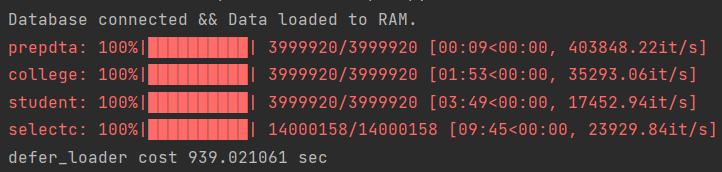
\includegraphics[width=0.6\textwidth]{pic/def.png}}

\subsubsection{异步插入}
\begin{lstlisting}[language=python]
async def async_loader(self):
    with open(conf, 'r', encoding='utf-8') as cfg:
        conf = yaml.safe_load(cfg)
    conn = await asyncpg.connect(host=conf['host'], port=conf['port'],
                                 user=conf['user'], password=conf['pwd'],
                                 database=conf['db'])
    # prepare data
    await conn.execute('BEGIN TRANSACTION;')
    await conn.execute('SET CONSTRAINTS ALL DEFERRED;')
    await conn.executemany('''INSERT INTO project1.college(name, eng_name)
                        	  SELECT $1, $2
                        	  ON CONFLICT DO NOTHING;''', atqdm(college))
    # similar for student info and course selection
    await conn.execute('COMMIT;')
\end{lstlisting}
\vspace{-3em}\par
此时耗时进一步缩短,相比于上一项再次提升约45.15\%,速度达到了平均42718条/秒。然而,异步对于本地数据库提升远不如连接云数据库时带来的提升比例大:如果提供一个网络服务,同时维护很多网络连接,并且每个网络连接都在操作数据库,这个异步过程就非常有意义,它会把数据操作过程本来应该阻塞等待的时间用来处理其它网络连接。\\\vspace{.3em}

\centerline{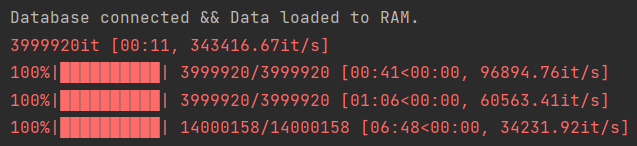
\includegraphics[width=0.6\textwidth]{pic/async.png}}

\subsubsection{连接池}
\begin{lstlisting}[language=python]
async def pool_loader(self, conf='./user.yml'):
    # data
    seq = 0
    for stu in tqdm(self.cdata):
        if seq == 500000:
            seq = 0
            college.append(college_seq.copy())
            stu_info.append(stu_info_seq)
            stu_sel.append(stu_sel_seq)
            college_seq.clear()
            stu_info_seq.clear()
            stu_sel_seq.clear()
        # preparing data packages (500000 students/pkg)
        seq += 1
    college.append(college_seq)
    stu_info.append(stu_info_seq)
    stu_sel.append(stu_sel_seq)
    self.cur.execute('BEGIN TRANSACTION;')
    self.cur.execute('SET CONSTRAINTS ALL DEFERRED;')

    conf = yaml.safe_load(open(conf, 'r', encoding='utf-8'))
    async with asyncpg.create_pool(host=conf['host'], port=conf['port'],
                                   user=conf['user'], password=conf['pwd'],
                                   database=conf['db']) as pool:
        async with pool.acquire() as cur:
            async for seq in atqdm(college):
                await cur.executemany('''INSERT INTO project1.college(name, eng_name)
                                    	 SELECT $1, $2
                                    	 ON CONFLICT DO NOTHING;''', seq)
            # similar for student info and course selection
\end{lstlisting}
\vspace{-3em}\par
在异步插入的基础上应用连接池能进一步提升速度。传统的使用多个连接进行插入会伴随大量的建立、断开连接开销,而上节异步的真正优势体现在高并发或者说并行插入。而连接池实现了连接的复用,正好弥补了上面的缺陷,两者配合,我们将学生数据按50万人/份进行打包,对每个包分别进行批处理插入,综合了以上探究的加速方法的所有优势,最终插入($3999920\times 2+14000158$)条数据总耗时仅216秒,平均每秒插入10.2万条记录,性能约为异步插入的2.38倍。\\\vspace{.3em}

\centerline{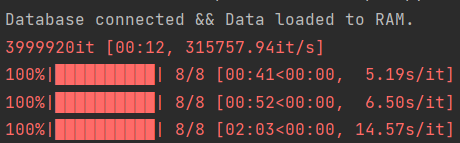
\includegraphics[width=0.4\textwidth]{pic/pkg50w.png}}

下表总结了各方法在插入选课数据(14000158条)时的耗时,由于其数据量较大且DBMS行为统一(无较多的ON CONFLICT DO NOTHING情况),能较好的代表其性能。表中相对提升指应用每项技术相比于不使用所带来的提升,综合性能是此项速度与传统插入的对比。
\begin{table}[H]
\centering
\begin{tabular}{|c|c|c|c|c|c|c|}
\hline
                      & 传统     & 关闭自动提交    & 批处理        & 延迟检查      & 异步插入     & 连接池       \\ \hline
耗时 / s                & 6086   & 3855      & 1216       & 585       & 408      & 123       \\ \hline
速度 / $it\cdot s^{-1}$ & 657.16 & 1037.53   & 11504.03   & 23929.84  & 34231.92 & 113822.42 \\ \hline
相对提升                  & -      & 57.88 \%  & 1008.79 \% & 108.01 \% & 43.05 \% & 232.51 \% \\ \hline
综合性能                  & -      & 157.88 \% & 1750 \%    & 3641 \%   & 5209 \%  & 17320 \%  \\ \hline
\end{tabular}
\end{table}


\section{DML性能分析}
\subsection{插入条目(增)}

插入条目耗时主要源自以下几点:
\vspace{-.5em}
\paragraph{条件检查} 关系型数据库为了保证ACID中的一致性(Consistency),会在插入动作后检查新插入的条目是否满足所有设置的条件(这里主要指CHECK),显然,每次插入所需检查的项目越多,耗时越长。以下控制其余变量保持一致,演示不断增加CHECK的数目,并在Python段用逐条插入(开启自动提交)所导致的时间消耗增加。
\begin{lstlisting}
CREATE TABLE demo1 (
    val int,
    CONSTRAINT demo1_chk1 CHECK (val > 0),
    CONSTRAINT demo1_chk2 CHECK (val % 2 = 0),
    CONSTRAINT demo1_chk3 CHECK (val < 10000)
);
\end{lstlisting}
\vspace{-2em}
\begin{table}[!h]
\centering
\begin{tabular}{|c|c|c|c|c|}
\hline
              & No constraint & chk1 & chk1\&2 & chk1\&2\&3 \\ \hline
插入500条数据 (ms) & 3593          & 3649 & 3776    & 3778       \\ \hline
\end{tabular}
\end{table}

\paragraph{外键约束} 每插入一条数据都需要在外键所指向的表中对应列检查是否有对应条目,此检查又与外键所指向的表中条目数有关:总数据量越大,在其中寻找某一可能存在的外键耗时越多。但所幸PostgreSQL会自动为外键所指向的列设置index,减少了检查耗时。
\begin{lstlisting}
CREATE TABLE demo2 (
    val int,
    cid varchar(20)          -- case 1: no foreign key constraint
    REFERENCES demo3(id)     -- case 2: demo3 contains 2 items
    REFERENCES courses(cid)  -- case 3: courses contains 338 items
);

\end{lstlisting}
\vspace{-2.3em}
\begin{table}[!h]
\centering
\begin{tabular}{|c|c|c|c|}
\hline
              & 无外键  & Ref 2 items & Ref 338 items \\ \hline
插入500条数据 (ms) & 3529 & 3804        & 3818          \\ \hline
\end{tabular}
\end{table}

\paragraph{主键 / 唯一性约束} 此检查耗时与当前此表中的条目数量相关,已有的条目越多,检查插入后是否依然满足唯一性的耗时越长。在批量插入中,越晚插入的数据因为已有数据不断增多而插入速度变慢。另外,主键列由于存在index,较一般的unique约束插入慢,见下文分析。
\begin{lstlisting}
CREATE TABLE demo3 (
    cid varchar(20) UNIQUE
);
\end{lstlisting}
\vspace{-2.3em}
\begin{table}[!h]
\centering
\begin{tabular}{|c|c|c|c|}
\hline
数据量(原有 $\to$ 插入后)        & 0 $\to$ 500 & 501 $\to$ 1000 & 1000 $\to$ 1500 \\ \hline
插入500条数据 (ms) & 3409        & 3614           & 3738            \\ \hline
\end{tabular}
\end{table}

\paragraph{Index更新}
当对表中的数据进行增加、删除和修改的时候,索引也要动态的维护,因此会降低数据的维护(增删改)速度。这也是我们需要避免在频繁修改数据的表中建立index的原因。
\begin{lstlisting}
CREATE TABLE demo4 (
    val1 int,
    val2 int
);
CREATE INDEX demo4_idx1 ON demo4 (val1);  -- for comparation
CREATE INDEX demo4_idx2 ON demo4 (val2);  -- for comparation
\end{lstlisting}
\vspace{-2.3em}
\begin{table}[!h]
\centering
\begin{tabular}{|c|c|c|}
\hline
              & 无index & 2 indexes \\ \hline
插入500条数据 (ms) & 3746   & 3898      \\ \hline
\end{tabular}
\end{table}

\subsection{删除条目(删)}
delete操作一般使用WHERE做限定词,这部分的耗时类似于查询(见下文分析);另外对于被指向的外键表中的数据,一般需要加上CASCADE进行级联删除。
\begin{lstlisting}
ALTER TABLE project1.learnt
    DROP CONSTRAINT learnt_sid_fkey;
ALTER TABLE project1.learnt
    ADD FOREIGN KEY (sid) REFERENCES project1.student (id)
        ON DELETE CASCADE;
        
DELETE FROM project1.student
WHERE sex = 'F'
  AND id BETWEEN 11000020 AND 11080020;
\end{lstlisting}
\vspace{-2.3em}
\par 此时的删除学生操作会将该学生的学习记录级联删除,执行删除语句的返回结果为\textit{40,220 rows affected in 1 s 591 ms}。
\subsection{查询条目(查)}

\paragraph{子查询} 子查询的设计会较大程度上的影响DBMS的性能,因为与其余常规查询操作不同,子查询一般无法被优化器综合性的优化进整体查询中。
\begin{lstlisting}
SELECT s.id, s.name
FROM project1.student s
WHERE s.college = (SELECT id FROM project1.college WHERE college.name = '格兰芬多')
  AND s.sex = 'M';
\end{lstlisting}
\vspace{-2em}
\par 在查询格兰芬多的所有男生信息时,使用子查询每次平均耗时0.308s,而查询书院编号及按编号查询数据的两个查询总耗时平均0.221s,这是因为类似于编程中的函数调用栈,当出现子查询时,查询器需要先保存上下文并跳转执行子查询,再将查询结果返回给“调用栈”的上一级查询任务。\\~\\
\centerline{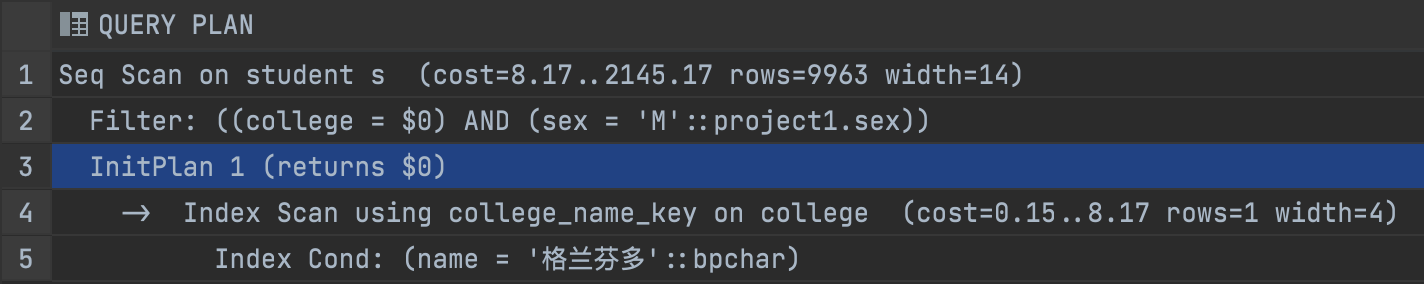
\includegraphics[width=0.9\textwidth]{dta/qp}}

\paragraph{索引} \par Index的设计能大大提升查询的性能。不使用index时,为了检查where子句中的条件,DBMS必须遍历整个表格中的所有行,并从众多列中选出其需要的部分,而为常用查询的条件部分设置index使得DBMS只需检查部分字段,大大减少了需要处理的信息量。
\begin{lstlisting}
SELECT sch_id
FROM project1.schedule
WHERE starting = 3
  AND ending = 4;
\end{lstlisting}
\vspace{-2em}
\par 在执行此查询时,该表上仅有数据库在设置主键列时自动添加的index,整表一共七个字段,而查询只涉及四个(且无完全包含查询所需字段的index),故需要提取每行的所有信息,耗时43ms。下面我们为查询涉及字段添加index,再次查询仅需15ms。此时DBMS在序列扫描数据时不需要提取全表信息,仅分析了sch\_time\_idx中包含的较少信息。更多关于索引的内容将于下文讨论。
\begin{lstlisting}
CREATE INDEX sch_time_idx ON project1.schedule (sch_id, starting, ending);
\end{lstlisting}
\vspace{-2em}
\paragraph{并行执行}
\par 并行化语句的执行过程会被规划器分发给多个后台进程去执行。 通过这种并行执行方式,PostgreSQL能充分发挥多核处理器的威力,从而让语句执行更快完成。通过并行化执行所能节省的时间根据数据库载体机的CPU核数的多寡而有所不同,在机器性能强大的情况下,并行化所能带来的性能提升可能非常可观。但是在查询任务数据量较少时,强制的并行化执行可能反而延长查询耗时——当每个进程所分配到的子任务规模较小时,创建worker的时间开销甚至大于执行查询的时间开销。
\par 通过下面的命令可以强行开启并行化执行模式,对比下例查询,使用1 worker时查询用时1.906s,并行化任务为其分配2 workers(如下图explain所示),耗时1.308s。
\begin{lstlisting}
SET force_parallel_mode = TRUE;
\end{lstlisting}
\vspace{-2em}
\begin{lstlisting}
SELECT course, COUNT(*)
FROM project1.learnt
GROUP BY course;
\end{lstlisting}
\vspace{-2em}
\centerline{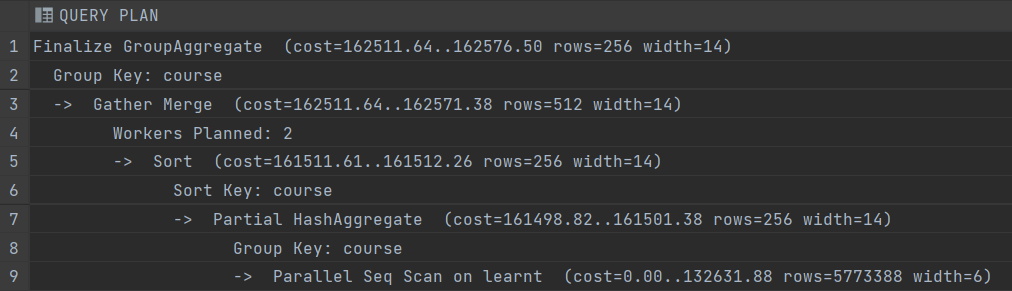
\includegraphics[width=0.8\textwidth]{dta/parall}}

\paragraph{where条件数} 若每层条件筛选后并不会大幅度减少剩余条目数量时,筛选条件越多,查询结果中剩余的项目分摊的执行时间越多,查询越慢。下例中标注的耗时指在原有条件的基础上增加此条件的耗时。
\begin{lstlisting}
SELECT sch_id
FROM project1.schedule
WHERE starting = 3 -- execution: 8ms
  AND ending = 4   -- execution: 9ms
  AND weekday = 3; -- execution: 11ms
\end{lstlisting}
\vspace{-2em}

\subsection{修改条目(改)}
一方面,关系型数据库要求修改后的数据依然保持所要求的\emph{一致性},并可能需要维护index,此部分检查的开销的分析见上文中“增”部分;另一方面则是WHERE限定词的查询开销。
\begin{lstlisting}
UPDATE project1.student
SET sex='M'
WHERE id BETWEEN 11000020 AND 11080020;
-- 39,781 rows affected in 162 ms
\end{lstlisting}
\vspace{-2em}

\section{DBMS-文件系统性能对比}
\subsection{大数据量}
这里以提供的选课数据csv为例,文件系统的查询使用Python,与数据库类似的,这里不将文件中内容读取至内存中,而是直接移动文件指针对磁盘中的信息进行处理(在DBMS中创建表,实际上相当于建立了数据到硬盘的一种映射,从而加速硬盘到内存的读写)。
考虑到DBMS在插入信息时需要向多表插入,且涉及大量检查,而文件系统的插入仅需对文件追加写入一行记录,删除与修改同理,两者本质差异过大而无较大的对比价值,因此本部分主要讨论数据的查询性能。
\par
DBMS以其优化器及性能著称。当使用文件系统查询时,或直接对文件进行读写,或将其模仿数据库中的结果加载进内存并进行查询,但均需要大量代码实现且需要手动优化。以下面模糊查询所有曾学过与C++相关的任何课程的学生为例:
\begin{lstlisting}[language=python]
@timer
def db_query():
    for _ in range(10):
        cur.execute('''SELECT s.id, s.name
                       FROM project1.learnt l
                                JOIN project1.student s ON l.sid = s.id
                                JOIN project1.course c ON l.course = c.cid
                       WHERE c.name ~ 'C\+\+';''')
    print(len(cur.fetchall()))

@timer
def fs_query():
    result_set = []
    for _ in range(10):
        f.seek(0)
        result_set.clear()
        cid = {
            c['courseId']
            for index, c in course_info.iterrows()
            if re.match(r'.*C\+\+', c['courseName'])
        }
        for stu in select_course:
            for c in cid:
                if c in stu[4:]:
                    result_set.append((stu[3], stu[0]))
                    break
        print(len(result_set))
\end{lstlisting}
\vspace{-3em}

\begin{figure*}[!h]
	\centering
	\begin{subfigure}[b]{0.3\textwidth}
		\centerline{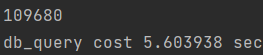
\includegraphics[height=1.1cm]{./dta/dbquery.png}}
		\caption{数据库查询}
	\end{subfigure}
	\qquad\quad
	\begin{subfigure}[b]{0.3\textwidth}
		\centerline{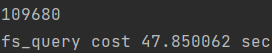
\includegraphics[height=1.1cm]{./dta/fsquery.png}}
		\caption{文件系统查询}
	\end{subfigure}
	\label{fig:visual_smap}
\end{figure*}

\par 上图所示进行十次查询并计时的结果,查询结果109680项。其中数据库每次查询平均耗时0.56s,仅为文件系统查询(平均耗时4.79s)的11.7\%。查看DBMS的查询规划可以发现,其用了如Hash join、Parallel sequence scan等技术节省时间,而在代码量相似的实现文件系统查询时仅相当于多个Sequence scan的嵌套。事实上,查询越复杂(指必要性上的复杂,而非故意将查询方式写得复杂而难以优化),DBMS的性能优势越明显(尤其是当能应用包括后面讨论的Index技术时),简单的查询可能已经难以进一步优化,性能将与文件系统相近。\\~\\
\centerline{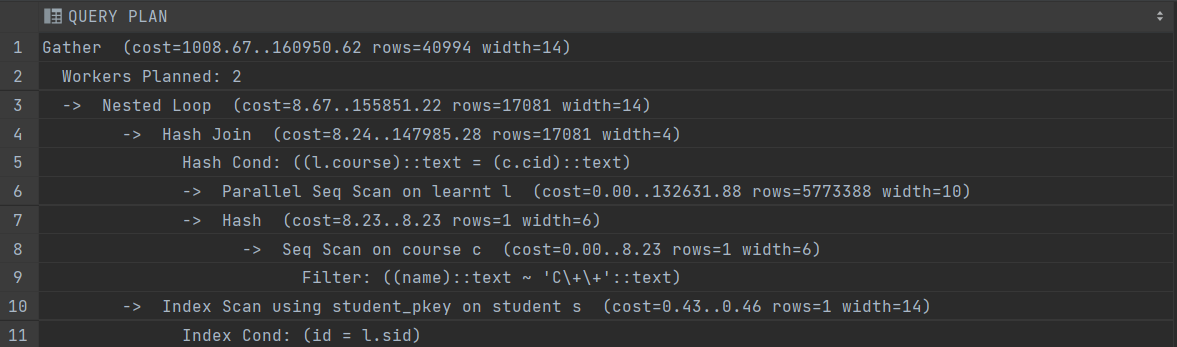
\includegraphics[width=0.9\textwidth]{dta/queryp}}

\subsection{小数据量}
以下展示基于题目提供的课程信息json文件,文件系统部分使用Python中的Pandas库处理。
\begin{lstlisting}[language=python]
@timer
def db_query():
    for _ in range(10):
        cur.execute('''SELECT DISTINCT cid
                       FROM project1.course
                       WHERE credit > 2;''')
    print(len(cur.fetchall()))

@timer
def fs_query():
    result_set = set()
    for _ in range(10):
        result_set.clear()
        for index, c in cif.iterrows():
            if c['courseCredit'] > 2:
                result_set.add(c['courseId'])
    print(len(result_set))
\end{lstlisting}
\vspace{-2em}
\par 上例重复十次查询所有计算机系开设的课程的列表,数据库耗时0.298s,文件系统耗时0.296s,可见即使是在运行速度较慢的Python中,依然能以微弱的优势领先数据库。这是由于小文件的遍历开销相对不大,而对于数据库的每次查询都有对任务的优化规划、SQL的语法检查、用户权限检查等环节的额外开销,因此查询耗时总耗时接近甚至超过文件系统的查询。

\par
数据库的安全性及完善的检查机制是文件系统所远不能及的,但也正是其一系列复杂的流程(语法检查、权限验证)为查询带来了一定的额外开销。当数据量大时,此开销相比于查询开销的比例极小,可以忽略不计,且一系列的优化(哈希、缓存、并行等)大大提升了查询效率;而对于极小的数据量,直接遍历文件已经作为较优的解决方案,DBMS在规划后可能给出的也是Seq scan的方案,但上述额外开销反而导致耗时较多。但从实际应用中来讲,应用数据库所存储的信息一般至少上千条,且查询的分摊总条目数也远大于遍历依然能跑赢优化的边界数量,也即平均角度上,使用数据库的查询性能是远优于文件系统的;且现实应用离不开数据库带来的一系列完善的检查及权限机制,数据库的优势依然是文件系统无法比拟的。\\~\\
\centerline{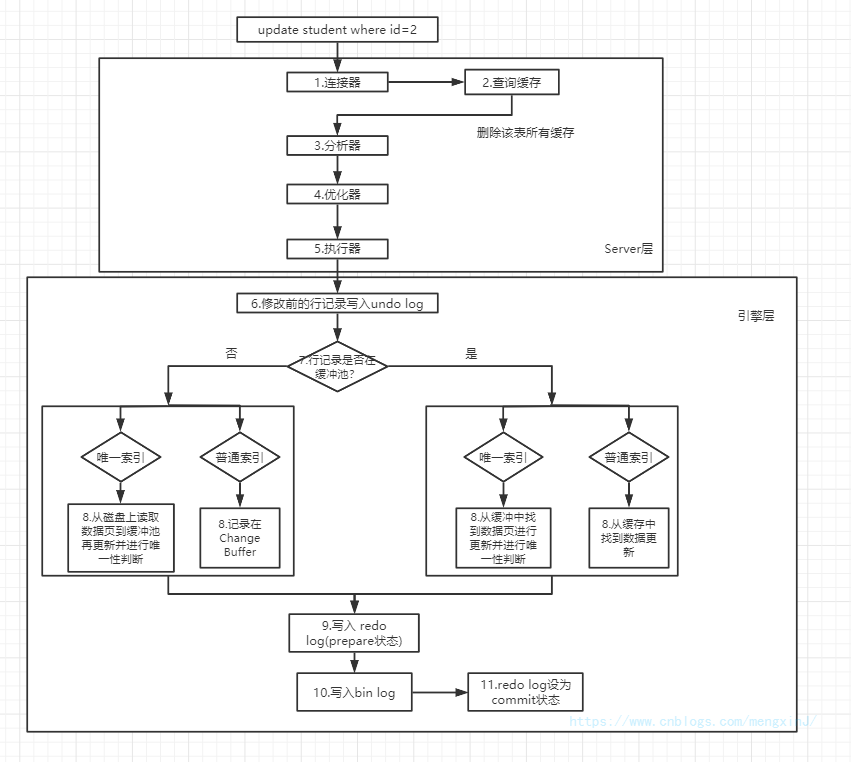
\includegraphics[width=0.8\textwidth]{pic/qry}}
\scriptsize
\centerline{InnoDB存储引擎的SQL操作过程\textsuperscript{\cite{m-2020}}}
\normalsize

\section{附加项}

\subsection{高并发及事务管理}
\subsubsection{高并发}
支持百万级别的高并发大数据流量已成为现代数据库系统的设计性能标准。在第二部分的最后,我们通过异步使用连接池,利用了数据库的高并发支持,在约两分钟的时间段内,数据库持续承受住了20个连接的写入操作。关于高并发的一个常见问题是\emph{死锁}。“加锁(Locking)是数据库在并发访问时保证数据一致性和完整性的主要机制。任何事务都需要获得相应对象上的锁才能访问数据,读取数据的事务通常只需要获得读锁(共享锁),修改数据的事务需要获得写锁(排他锁)。当两个事务互相之间需要等待对方释放获得的资源时,如果系统不进行干预则会一直等待下去,也就是进入了死锁(deadlock)状态。”\textsuperscript{\cite{dong-2021}}\\~\\
\centerline{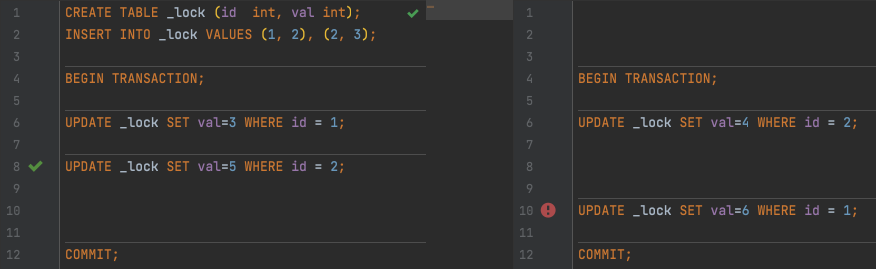
\includegraphics[width=0.8\textwidth]{sp/lkdemo}}
\par 上图尝试在不同事务中以不同的顺序修改数据,首先在左事务中修改id为1的数据,此部分被加锁、右事务修改id为2的数据,同样加锁;第二步让左事务修改id为2的数据,但此时DBMS为避免脏写,已经为其加上写锁,因此左事务的进程需要等待右事务结束以释放写锁;在左事务的等待状态中,右事务修改被左事务添加写锁的数据,此时右事务也进入等待状态;注意到左事务一直在等待右事务结束以释放写锁,而右事务也在等待左事务释放写锁以执行命令并结束,两个事务进入了互相等待对方资源的状态,这种等待是无限的。但现在大部分数据库都能在等待一段时间后检查出死锁,并做出\emph{终止一个事务并让另一个事务成功执行}的调度(如下图)。但是一个事务长期等待另一个事务释放资源并不会引起DBMS的介入。\\~\\
\centerline{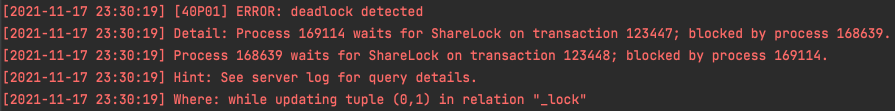
\includegraphics[width=0.85\textwidth]{sp/dlock}}


\subsubsection{事务管理}
事务管理主要为RDBMS提供了\emph{原子性 (Atomicity)、一致性 (Consistency)、隔离性 (Isolation)和持久性 (Durability)}这四大特性\textsuperscript{\cite{silberschatz-2010}}。
\paragraph{原子性} 指一个事务块中的所有事件或全部成功执行,或全不执行,即在中间任何一个事件失败时需要回滚指事务开始时的状态。在事务块中遇到第一个错误后,Postgres会忽略后面的命令,直至执行一次\textbf{ROLLBACK}回滚至事务开始时的状态,或执行\textbf{COMMIT}并由DBMS丢弃此事务块的所有影响。此外,即使所有操作成功执行,用户也可使用ROLLBACK取消所做修改。
\begin{figure*}[!h]
	\centering
	\begin{subfigure}[b]{0.3\textwidth}
		\centerline{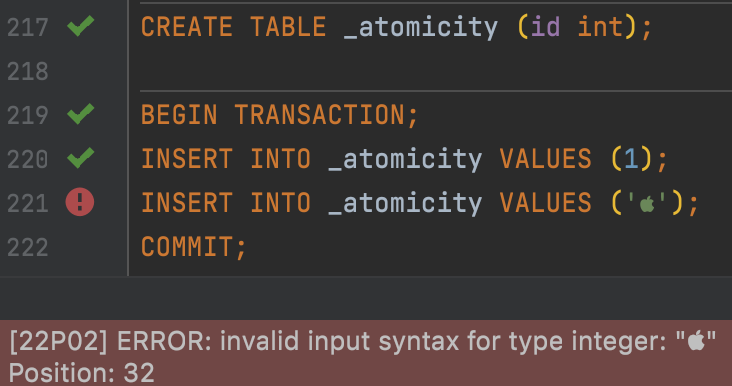
\includegraphics[height=2.7cm]{./sp/trs1}}
		\caption{事务块中出现错误}
	\end{subfigure}
	\\
	\begin{subfigure}[b]{0.3\textwidth}
		\centerline{
\includegraphics[height=0.7cm]{./sp/trs2}}
		\caption{提示当前事务块所有会被取消}
	\end{subfigure}
	\\
	\begin{subfigure}[b]{0.9\textwidth}
		\centerline{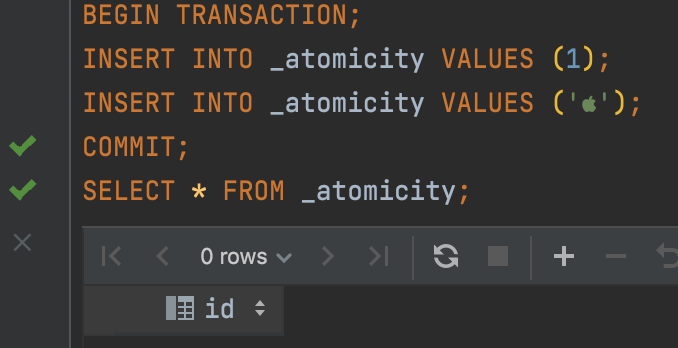
\includegraphics[height=2.7cm]{./sp/trs3}}
		\caption{执行COMMIT,此时DBMS取消了事务中的操作,查询结果所示与事务开始前状态一致}
	\end{subfigure}
	\\
	\begin{subfigure}[b]{0.9\textwidth}
		\centerline{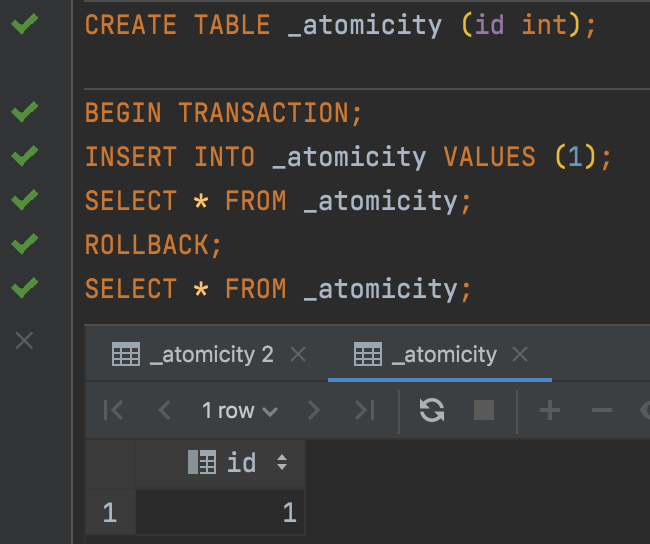
\includegraphics[height=2.75cm]{./sp/trs4}\qquad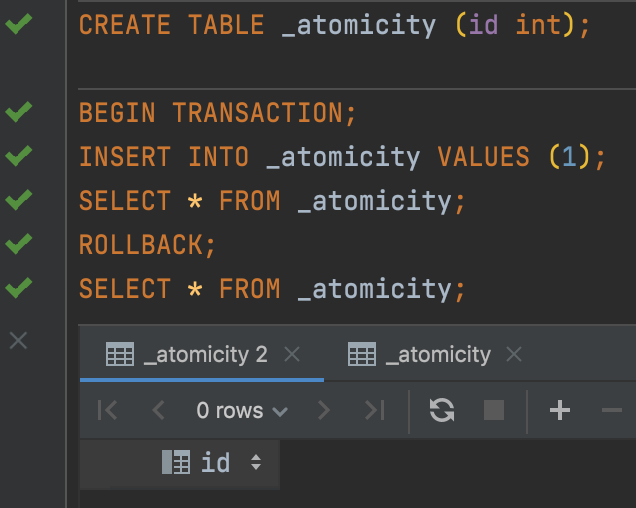
\includegraphics[height=2.75cm]{./sp/trs5}}
		\caption{左图示成功插入一条数据,执行回滚后再次查询,结果与事务开始前一致}
	\end{subfigure}
\end{figure*}

\paragraph{一致性} 报告第二部分插入数据即利用了此特性。出于各种原因,人们可能不关心某件事中间过程的高度一致,而仅要求事件前后均满足各种限制即可。“在事务开始之前和事务结束以后,数据库的完整性没有被破坏。这表示写入的资料必须完全符合所有的预设约束、触发器、级联回滚等。”\textsuperscript{\cite{acid-wiki}}
\begin{figure*}[!h]
	\centering
	\begin{subfigure}[b]{0.9\textwidth}
		\centerline{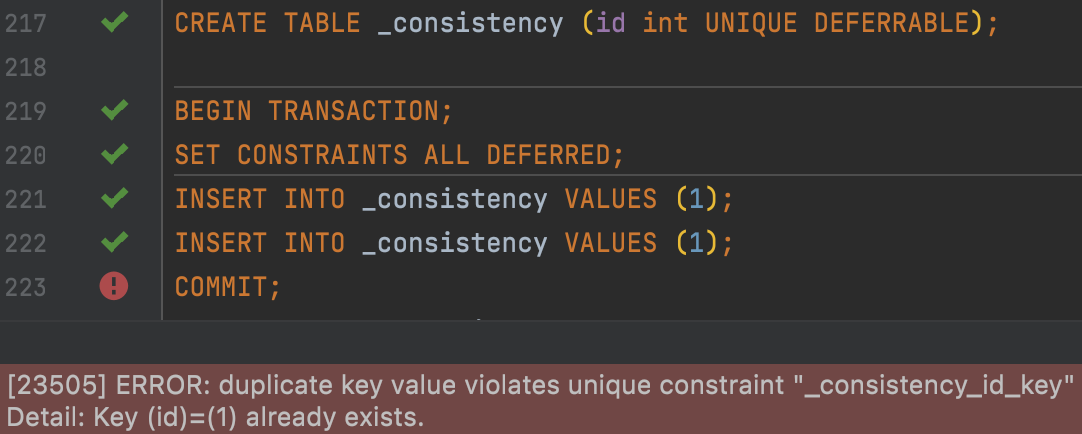
\includegraphics[height=2.7cm]{./sp/trs6}\qquad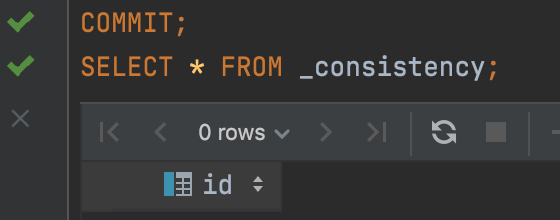
\includegraphics[height=2.7cm]{./sp/trs7}}
		\caption{延迟检查使事务块中可违反一些约束,而在COMMIT前会检查一致性并报错}
	\end{subfigure}
\end{figure*}

\paragraph{隔离性} “数据库允许多个并发事务同时对其数据进行读写和修改的能力,隔离性可以防止多个事务并发执行时由于交叉执行而导致数据的不一致。事务隔离分为不同级别,包括未提交读(read uncommitted)、提交读(read committed)、可重复读(repeatable read)和串行化(serializable)。”\textsuperscript{\cite{acid-wiki}}
\par 以下测试均在DataGrip中使用console建立一个连接,并在CLI中使用另一角色登录并修改数据,以此模拟并发读写。
\subparagraph{读已提交} 下面的实验展示在读已提交的隔离级别中,一个查询只能看到查询开始前已提交的数据(查询开始瞬间的数据库快照),无法看到未提交或查询期间由其他事物提交的数据,但查询可看见自身事务中之前执行的更新。读已提交不会导致\emph{脏读}(即一个事务读取了另一个未提交的事务写入的数据),同时也是PostgreSQL的默认隔离级别。但读已提交也可能造成不可重复读,即同一事务中两个相邻查询返回的结果可能不同,这是因为在两次查询开始的间隔中可能有其他事务被提交。
\begin{lstlisting}
conn1=# CREATE TABLE _isolation (id  int, val int);
conn1=# SELECT * FROM _isolation;
 id | val 
----+-----
(0 rows)

conn1=# BEGIN TRANSACTION;
conn1=# SET TRANSACTION ISOLATION LEVEL READ COMMITTED;
conn2=# BEGIN TRANSACTION;
conn2=# INSERT INTO _isolation VALUES (2, 1);
conn1=# SELECT * FROM _isolation;
 id | val 
----+-----
(0 rows)

conn2=# COMMIT;
conn1=# SELECT * FROM _isolation;
 id | val 
----+-----
  2 |   1
(1 row)
\end{lstlisting}
\vspace{-2em}

\subparagraph{可重复读} 与读已提交的一个非常相似的隔离级别是可重复读,其只允许读取已提交数据,且一个事务两次读取一个数据项期间,不允许其他事务更新该数据,即一个可重复读事务中的查询可以看见在事务中第一个非事务控制语句开始时的一个快照。但其与读已提交一样,依然可能出现幻读。
\begin{lstlisting}
conn1=# CREATE TABLE _isolation (id  int, val int);
conn1=# BEGIN TRANSACTION;
conn1=# SET TRANSACTION ISOLATION LEVEL REPEATABLE READ;
conn2=# BEGIN TRANSACTION;
conn2=# INSERT INTO _isolation VALUES (2, 1);
conn2=# COMMIT;
conn1=# SELECT * FROM _isolation;
 id | val 
----+-----
(0 rows)

conn1=# COMMIT;
conn1=# SELECT * FROM _isolation;
 id | val 
----+-----
  2 |   1
(1 row)
\end{lstlisting}
\vspace{-2em}

\subparagraph{可串行化} 是四种隔离级别中唯一避免了\emph{幻读}\footnote{一个事务开始后,需要根据数据库中现有的数据做一些更新,于是重新执行一个查询,返回符合查询条件的行,这时发现这些行因为其它最近提交的事务而发生了改变,导致现有事务如果再进行下去可能发发生逻辑上的错误。}的级别,也即是最高的事务隔离级别,在该级别下,事务串行化顺序执行,可以避免脏读、不可重复读与幻读\footnote{不可重复读对应的是修改,即UPDATE操作;而幻读问题对应的是INSERT操作。}。但是这种事务隔离级别效率低下,比较耗数据库性能,不常用。

\subparagraph{读未提交} 允许读取未提交的数据,是SQL允许的最低一致性级别。可能导致脏读、不可重复读以及幻读(但对于PostgreSQL,此级别的行为与读已提交相同,因为DBMS内部实际上只实现了另外三种隔离级别)。另外,以上四种隔离级别均不允许脏写。


\paragraph{持久性} 事务块成功结束后,对数据的修改就是永久的,即便系统故障也不应丢失。如下图所示,将postgres.service强制突然kill掉,模拟系统突然故障,此后重新启动服务,检查数据库存储条目与kill前一致(kill前已结束事务)。\\~\\
\centerline{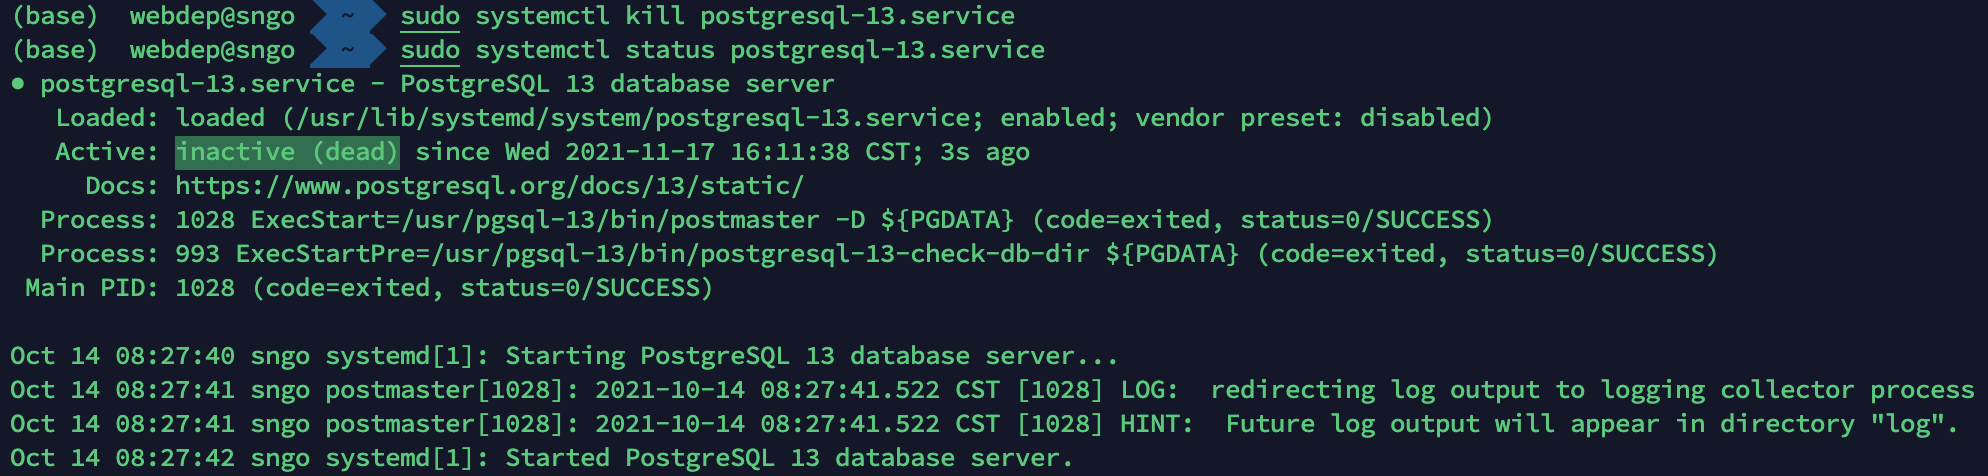
\includegraphics[width=0.7\textwidth]{sp/kill}}
\subsection{用户权限管理}
DBMS最有用的特性之一便是其完善健全的用户权限管理机制。考虑数据库的日常使用场景,为不同的用户(更正确的说,角色)提供不同级别、不同类型的权限是很有必要的。
\subsubsection{角色 (Roles)}
PostgreSQL为管理“用户”及其权限提供了\emph{角色}机制,在此机制下,“用户”、“用户组”是同一个概念,这点与MySQL等数据库的机制有十分关键的区别。
\par 
用户与用户组实际上都作为“角色”存储在\emph{pg\_roles}数据库中,自然,他们拥有同样数目的属性。使用DBMS的用户拥有一个\emph{登录角色 (login role)},同时,它可以从另一个角色继承权限,成为其 \emph{成员角色 (member role)},同时,拥有一些成员角色的角色现在被命名为 \emph{组角色 (group role)}。一般来说,出于安全性考虑,组角色不授予登录权限\textsuperscript{\cite{be-2017}},因为组角色被设计成一个权限集合,以便于管理多个用户的权限,而不是作为一个真正需要登录权限的用户的角色。从Postgres 8开始,我们可以用create user来明确指出创建的角色是一个普通的用户账户,其默认赋予可登录权限;而create role所创建的角色被Postgres认为可能作为组角色,默认是不具登陆权限 (cannot login) 的\textsuperscript{\cite{obe-2017}},这也是Postgres中“用户”与“用户组”最核心的区别。\\
\begin{figure*}[!h]
	\centering
	\begin{subfigure}[b]{0.8\textwidth}
		\centerline{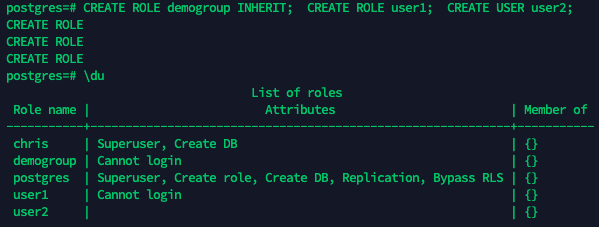
\includegraphics[height=2.5cm]{./pic/role1.png}\quad 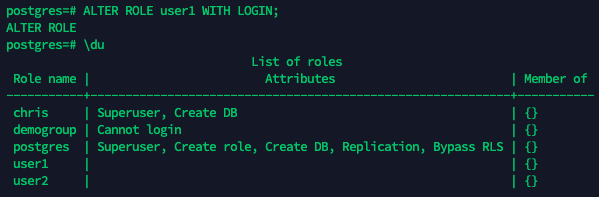
\includegraphics[height=2.5cm]{./pic/role2.png}}
		\caption{创建两个可登录角色、一个不可登录角色(组角色;\emph{INHERIT}关键词可省略)}
	\end{subfigure}
	\\~\\
	\begin{subfigure}[b]{0.8\textwidth}
		\centerline{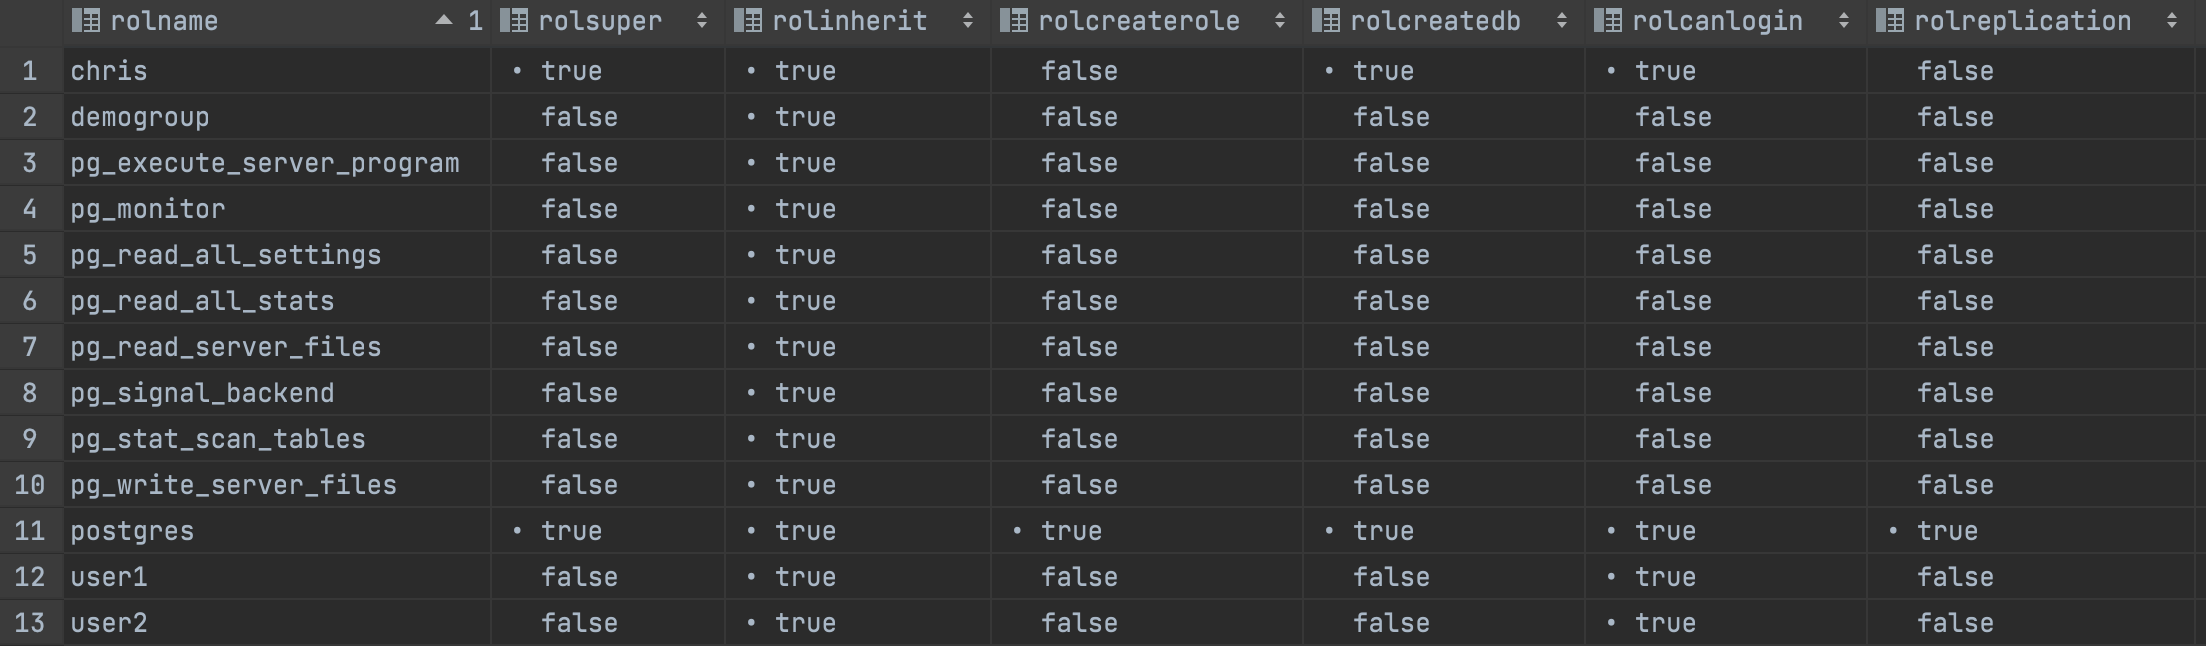
\includegraphics[width=\textwidth]{./pic/pgr.png}}
		\caption{SELECT * FROM  pg\_roles;}
	\end{subfigure}
	\\~\\
	\hspace{-2.3cm}
	\begin{subfigure}[b]{0.5\textwidth}
		\centerline{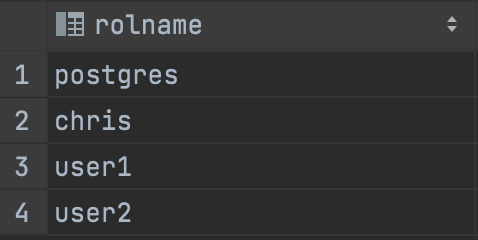
\includegraphics[height=2.5cm]{./pic/pgrw.png}}
		\caption{SELECT * FROM pg\_roles WHERE rolcanlogin;}
	\end{subfigure}
	\quad
	\begin{subfigure}[b]{0.3\textwidth}
		\vspace{-2.5cm}
		\centerline{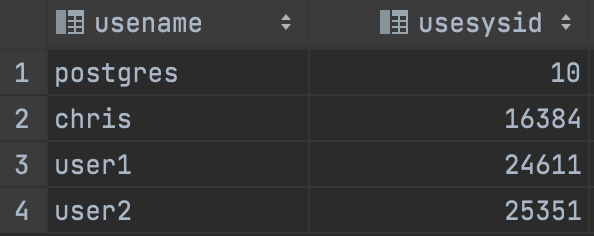
\includegraphics[height=2.5cm]{./pic/pgu.png}}
		\caption{SELECT * FROM  pg\_user;}
	\end{subfigure}
\end{figure*}

\indent 上图 (b) 和 (d) 
示PostgreSQL 13.3中依然有“用户”的概念,但其只是作为\emph{可登录角色}的别名\textsuperscript{\cite{psqldoc, unknown-author-2014}}。
\centerline{CREATE USER [usr] = CREATE ROLE [usr] WITH LOGIN}
\par
尽管Postgres中的“组角色”也可以作为另一个组角色的成员角色,这种嵌套关系是不限层数的,但一般为了安全性,DBA需要避免过多层组角色的继承以避免无意的为不该拥有某权限的角色授权。

% 越权与权限授予、收回
\subsubsection{权限授予}
当DBMS收到一条请求后,在首先检查其语法无误后,DBMS会检查发送请求的角色(\emph{role})及其是否有相应权限。如下图所示,如果发送SQL请求的角色没有对应权限,DBMS将拒绝该请求。为角色授权的语法如下\textsuperscript{\cite{unknown-author-2021}}:
\begin{lstlisting}
GRANT { { SELECT | INSERT | UPDATE | DELETE | TRUNCATE | REFERENCES | TRIGGER }
    [, ...] | ALL [ PRIVILEGES ] }
    ON { [ TABLE ] table_name [, ...]
         | ALL TABLES IN SCHEMA schema_name [, ...] }
    TO role_specification [, ...] [ WITH GRANT OPTION ]
\end{lstlisting}
\vspace{-2em}

\centerline{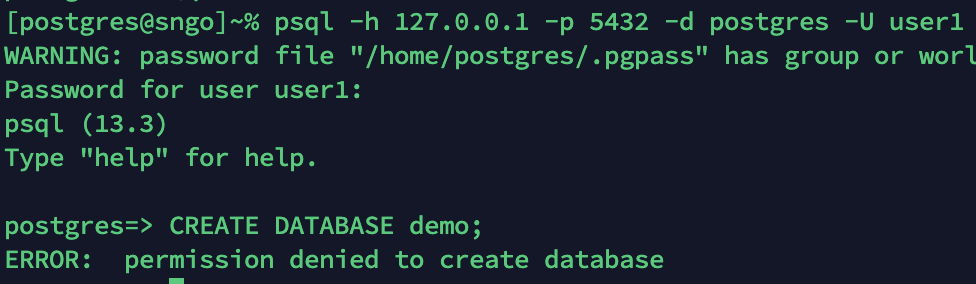
\includegraphics[width=0.65\textwidth]{./pic/nopriv.png}}
\vspace{1em}
\centerline{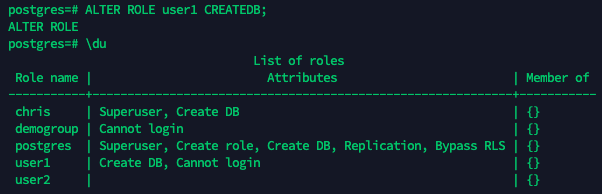
\includegraphics[height=2.5cm]{./pic/cdb.png}\quad 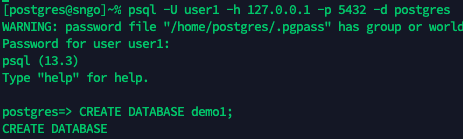
\includegraphics[height=2.5cm]{./pic/u1cdb.png}}

\par
特别地,一个“对象”(schema、table等)的所有者自然拥有该对象的所有权限。然而,作为对象的所有者并不意味着其是该对象的所有子对象的所有者(见下页图(c))。比如,如果一个角色创建并拥有一个数据库,而另一个角色在此数据库中创建了一个schema,则该对象默认并没有权限去访问此schema,但可以直接删除它。
\par
只有权限的拥有者(其必须同时拥有该权限的grant权限)可以将权限授予其他角色,而有些权限只能由对象的拥有者持有,如DROP和ALTER。另外,当授予一个角色时,可以通过添加WITH GRANT OPTION来允许该角色授予其他角色。
\par
当创建一个新的数据库时,DBMS会默认创建一个名为\emph{public}的schema,并将该schema的访问权授予一个名为public的角色。所有新的用户和角色都被默认授予public角色中的所有权限,因此所有人都可以在此public schema中创建对象。\\~\\
\centerline{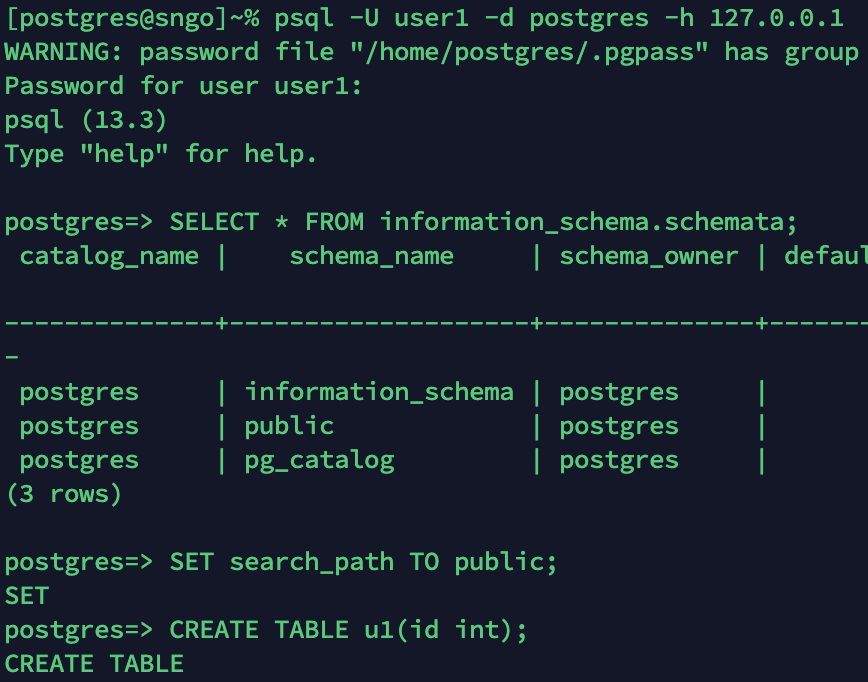
\includegraphics[width=0.6\textwidth]{./pic/mov.png}}
\begin{figure*}
	\centering
	\begin{subfigure}[b]{0.8\textwidth}
		\centerline{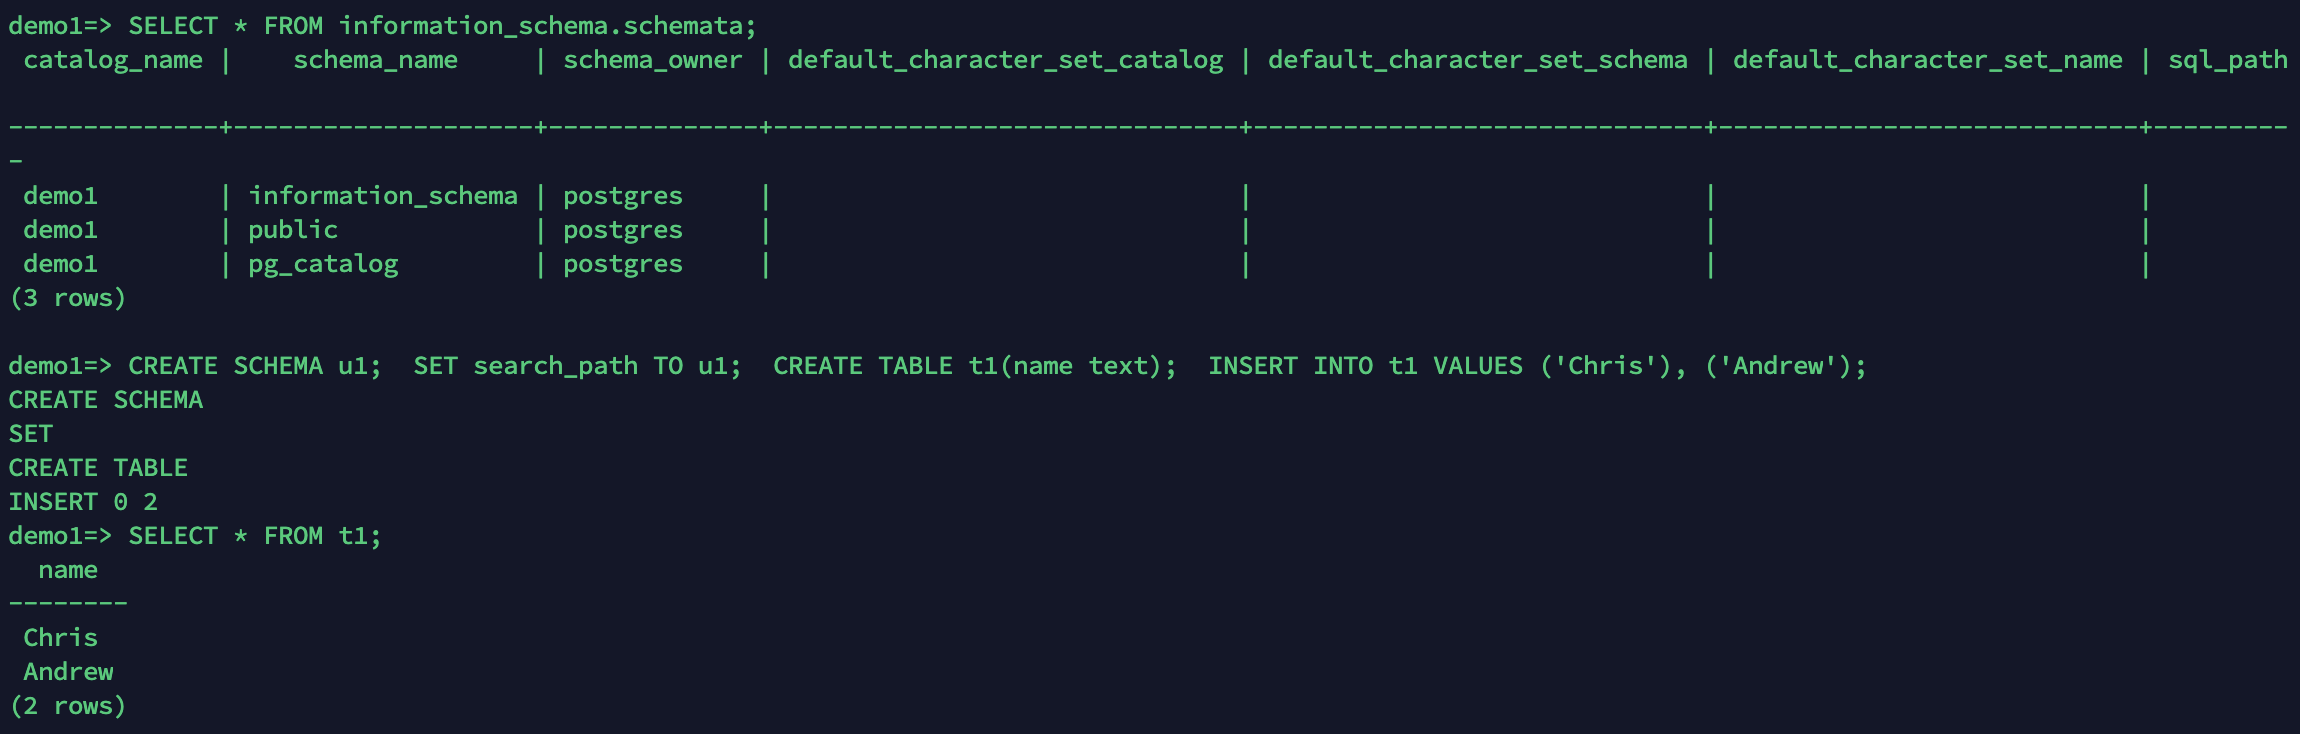
\includegraphics[height=3.6cm]{./pic/ins.png}}
		\caption{对象的创建者自动拥有该对象的所有权限}
	\end{subfigure}
	\\~\\
	\begin{subfigure}[b]{0.8\textwidth}
		\centerline{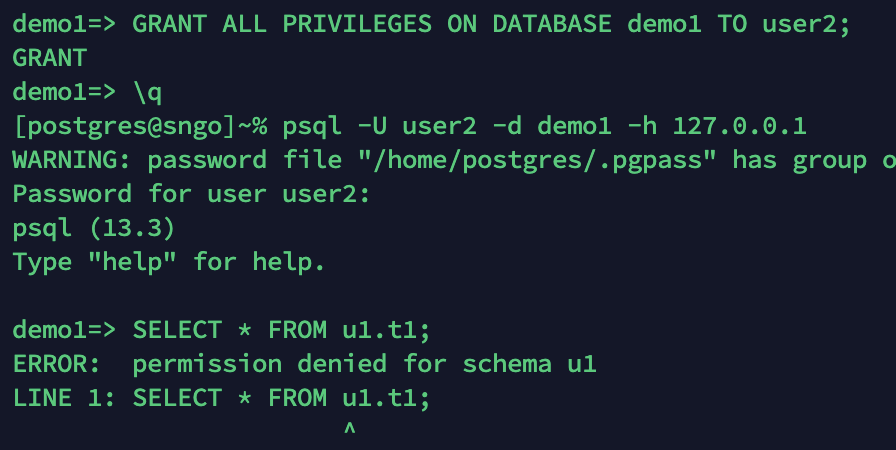
\includegraphics[width=0.6\textwidth]{./pic/grdb_nsch.png}}
		\centerline{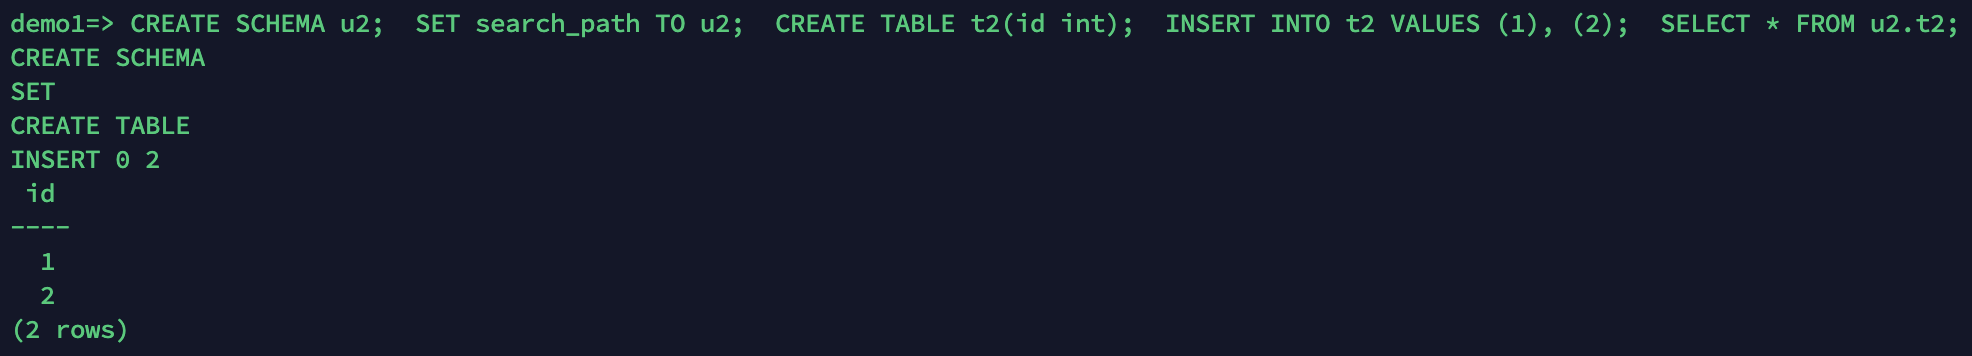
\includegraphics[width=0.6\textwidth]{./pic/u2.png}}
		\caption{角色被授予某数据库的所有权限后,依然不能访问特定的schema(除public外,由其他角色创建),但可以对数据库进行其他操作}
	\end{subfigure}
	\\~\\
	\begin{subfigure}[b]{0.8\textwidth}
		\centerline{\includegraphics[width=\textwidth]{./pic/nvsb.png}}
		\caption{user2在user1所拥有对数据库中创建的schema对user1不可见}
	\end{subfigure}
	\\~\\
	\begin{subfigure}[b]{0.8\textwidth}
		\centerline{\includegraphics[width=0.6\textwidth]{./pic/ddpu1.png}}
		\caption{user1未被授予schema u2的相关权限,但因为其拥有整个数据库,因此可以直接将其drop}
	\end{subfigure}
	\label{fig:visual_smap}
\end{figure*}
\pagebreak


\subsubsection{撤回权限}
收回权限的语法与授权的语法类似:
\begin{lstlisting}
REVOKE [ GRANT OPTION FOR ]
    { { SELECT | INSERT | UPDATE | DELETE | TRUNCATE | REFERENCES | TRIGGER }
    [, ...] | ALL [ PRIVILEGES ] }
    ON { [ TABLE ] table_name [, ...]
         | ALL TABLES IN SCHEMA schema_name [, ...] }
    FROM role_specification [, ...]
    [ CASCADE | RESTRICT ]
\end{lstlisting}
\vspace{-2em}
\centerline{\includegraphics[width=0.5\textwidth]{pic/rvk}}
\par 在Postgres中较为特殊的一点是,删除角色时,一般不能直接删除,而要先将该角色被授予的所有权限收回,并转移其拥有的对象的所有权。\\~\\
\centerline{\includegraphics[width=0.7\textwidth]{pic/fail2dr}}

\subsubsection{组角色}
在前两小节的演示角色的图(a)中我们创建了一个名为\emph{demogroup}的组角色, 现用角色\textit{postgres}创建一个数据库,并将其所有权限赋予给该组角色。注意我们至始至终没有给user1授予权限。接下来,通过\\
\centerline{GRANT [group\_role] TO [login\_role];}
命令将user1和user2加入demogroup的成员角色。下图演示了进入组角色的user1自动继承了组中所有权限,我们得以在不直接对user1授权的情况下使user1有权操作该数据库。\\~\\
\centerline{\includegraphics[width=0.7\textwidth]{./pic/grp.png}}
\centerline{\includegraphics[width=0.7\textwidth]{./pic/grgrp.png}}
\centerline{\includegraphics[width=0.7\textwidth]{./pic/grgrp2.png}}
\par 要删除一个组角色,执行DROP ROLE [group\_role]命令即可。在删除该组角色之后,它与其成员角色之间的关系将被立即撤销,而成员角色本身不受影响。需要注意的是,在删除前任何属于该组角色的对象都必须先被删除或者将对象的所有者转移给其它角色,与此同时,任何赋予该组角色的权限也都必须被撤消\textsuperscript{\cite{turing-2021}} 。
\subsubsection{文件系统用户权限管理}
文件系统可以通过改变文件的权限(以UNIX系OS为例,一般我们关注读、写、可执行权限)来达到类似的效果,通过系统自带的用户机制可以为不同用户、针对某个文件,分配不同的权限。\\~\\
\centerline{\includegraphics[width=0.55\textwidth]{pic/fsp}}
\par 上图演示在CentOS中使用root账号创建文件,并执行\textbf{chmod 600}命令使文件仅创建者可读写(如第一个ll所示),此时登录另一账号尝试读取文件,权限不足被拒;再次执行\textbf{chmod 666}对所有用户开放读写权限(如第二个ll所示),再次读取文件则成功显示内容。
\subsection{数据库索引及文件IO}
\subsubsection{数据库索引}
对于没有index的表的查询,DBMS需要将整行数据取出并在其中少数几个字段应用筛选器,这种操作是低效的。而为了能直接定位所需的记录,DBMS设计了\emph{索引}这种与文件相关联的附加的结构。常用的索引形式为B$^+$树及散列索引。
\par 当查询的限定字段被某一索引所包括时,DBMS首先查找索引,找出相应记录所在的磁盘块,再取出相应的(存储数据量较小的)磁盘块并在其中高效搜索\textsuperscript{\cite{silberschatz-2010}} 。但索引并非越多越好:一方面,创建索引和动态维护索引要耗费时间;另一方面,索引需要占物理空间,除了数据表占数据空间之外,每一个索引还要占一定的物理空间,如果要建立聚簇索引,那么需要的空间就会更大。


\par 在以下情况下使用索引能带来较优的效果\textsuperscript{\cite{silberschatz-2010}}:
\vspace{-1.5em}
\paragraph{\ding{172}} 频繁需要搜索的列;
\vspace{-1.5em}
\paragraph{\ding{173}} 主键列、唯一性约束、外键列等,强制该列的唯一性和组织表中数据的排列结构(PostgreSQL会自动为这些列设置索引);
\vspace{-1.5em}
\paragraph{\ding{174}} 连接表或检查被用作连接(join)的列,即一般指外键列;
\vspace{-1.5em}
\paragraph{\ding{175}} 经常需要进行范围搜索的列,可利用索引已排序的特性对数值进行连续搜索;
\vspace{-1.5em}
\paragraph{\ding{176}} 经常需要排序的列同样可利用索引已排序的特性减少排序步骤的耗时;
\vspace{-1.5em}
\paragraph{\ding{177}} 频繁作为限定条件的字段组合(列)。

\par 而以下情况使用索引的效果并不佳:
\vspace{-1.5em}
\paragraph{\ding{172}} 查询中很少使用或者参考的列不应该创建索引(对查询速度的优化场景较少,而DBMS多了储存与维护索引的时间、空间负担);
\vspace{-1.5em}
\paragraph{\ding{173}} 数据量较少的列不需要设置索引;
\vspace{-1.5em}
\paragraph{\ding{174}} 连接表或检查被用作连接(join)的列,即一般指外键列;
\vspace{-1.5em}
\paragraph{\ding{175}} Text, image, blob等数据类型的列不应该增加索引,因为这些列的数据量较大或取值很少;
\vspace{-1.5em}
\paragraph{\ding{176}} 需要频繁修改而较少需要检索的表:修改性能和检索性能互相矛盾,当增加索引时,会提高检索性能,但是会降低修改性能,当减少索引时,会提高修改性能,降低检索性能。\\~\\
\centerline{\includegraphics[width=0.6\textwidth]{sp/idx}}
\scriptsize
\centerline{SELECT * FROM project1.student WHERE id = 11080020; 这里id作为主键列已经设有index}
\normalsize

\par 以下查询所有与海洋相关的院系所开设的课程及教师。此时join中用到的连接列均有数据库默认加上的index,键入EXPLAIN ANALYSE命令分析可见大量\emph{hash join, hash cond, index scan, index cond}等,查询耗时0.368ms。
\begin{lstlisting}
SELECT c.name, t.name
FROM project1.course c
         JOIN project1.department d ON c.dept = d.id
         JOIN project1.class cls ON cls.course = c.cid
         JOIN project1.class_teacher ct ON ct.class = cls.id
         JOIN project1.teacher t ON t.id = ct.teacher
WHERE d.name ~ '海洋'
ORDER BY c.name, t.name;
\end{lstlisting}
\vspace{-2em}
\centerline{\includegraphics[width=0.85\textwidth]{sp/idxp}}

\par 下面通过对比能体现索引带来了极高的查询效率提升。对于查询语句\textbf{SELECT class FROM schedule WHERE weekday = 5},原始的无索引查询(如左下图)进行了序列扫描,需要取出表中所有信息,耗时0.281s,而通过\textbf{CREATE INDEX ON project1.schedule (weekday)}为WHERE限定列加上索引后,查询耗时仅为0.147s(如右下图),相比无索引查询节省了47.6\%的时间。\\~\\
\centerline{\includegraphics[height=4em]{sp/nid}\qquad\includegraphics[height=4em]{sp/id}}

\subsubsection{文件索引(数据结构)}
使用Python对无索引的课程信息文件十次检索学分大于2的课程,耗时0.525s:
\begin{lstlisting}[language=python]
def fs_query() -> set:
    result_set = set()
    for _ in range(10):
        result_set.clear()
        for index, c in cif.iterrows():
            if c['courseCredit'] > 2:
                result_set.add(c['courseId'])
    return result_set
\end{lstlisting}
\vspace{-2em}
\par 下面为相应条目创建索引\footnote{使用了GitHub上的B+树代码实现:adigan1310 / BPlus-Tree-Indexing}\textsuperscript{\cite{unknown-author-2017}}
\begin{lstlisting}[language=java]
Index idx = new Index();
idx.index("courseCredit", "course_info.json", "idx_course_info.bpt");
idx.searchindex("idx_course_info.bpt", "courseCredit > 2", " ");
\end{lstlisting}
\vspace{-2.3em}
\par 调用该封装好的函数如同使用SQL一样方便,首先需要对对应的字段创建索引,然后解析此索引并进行搜索,并加工searchindex函数返回的原始结果(相对于 SELECT *),十次搜索耗时0.319s,但考虑到JVM和Python interpreter的性能差异,该结果仅供参考。

\subsection{跨平台性能对比}
\paragraph{File system} \ding{172} CentOS 7.9.2009 (Python 3.8.8)\qquad\ding{173} macOS 12.0.1 (Python 3.8.10)
\vspace{-1.4em}
\paragraph{RDBMS} \quad\hspace{.276em}\ding{172} PostgreSQL 13.3\qquad\ding{173} MySQL 5.6.50\qquad\ding{174} SQLite 3.34.0
\par 数据均以相同结构存储在数据库中,而文件系统部分考虑到Java历史久远,JVM在各平台下的表现高度均一,仅能体现不同评测环境的硬件区别,故使用Python进行对比,使用Pandas库读取csv文件。以下是查询所有修完CS205的学生信息的平均耗时(文件系统重复十次查询取平均,数据库不预热;下表中数据库项均为execution + fetching,由于使用的均为云数据库,fetching time受网络环境延迟影响数值较大):
\begin{table}[!h]
\centering
\begin{tabular}{|c|c|c|c|c|c|}
\hline
          & macOS (Python) & CentOS (Python) & PostgreSQL & MySQL  & SQLite \\ \hline
平均耗时 (ms) & 1139           & 1271            & 345 + 112     & 317 + 107 & 359 + 120 \\ \hline
\end{tabular}
\end{table}

\par 注意到PostgreSQL在查询速度上略低于MySQL,这是因为PostgreSQL和MySQL均是基于MVCC机制 (Multi-Version Concurrency Control) 来保证事务的原子性和隔离性的,该模型将争用降低到最低限度以期减少操作的阻塞。PostgreSQL的实现和MySQL基于的InnoDB引擎的实现是目前公认的两大实现MVCC的方法。其主要区别在于Postgres在查询开始时为了避免脏读而存储的旧版本,其只是在元组的较旧版本上更新xmax,因此较旧版本的大小与相应的插入记录相同。而对于InnoDB,存储在Undo段中的对象版本通常小于相应的插入记录。这是因为仅将更改的值(即差分)写入UNDO日志。\textsuperscript{\cite{blue-2020}}而轻量级的SQLite相较于另外两种数据库,更接近于文件系统。文件系统的查询速度有细微差异,这可能是由于Python interpreter在不同系统上的实现略微不同以及不同系统对文件存储策略的不同造成的。
\par 本次测试中也注意到,数据库在第一次查询时耗时(345ms)远大于后续几次进行相同查询(30ms),这是由于DBMS的缓存策略相比起文件系统中实现的更加健全高效,在第一次将数据搬入缓存或内存中后,后续查询能有较高的缓存命中率。

\vspace{2em}
\footnotesize
\bibliographystyle{IEEEtran}
\bibliography{commondb}

\noindent \scriptsize{Disclaimer: All references used in this project are only for the purpose of guiding the direction of exploration and ensuring correctness, any code appearing in the referenced web pages has not been used directly, unless explicitly stated.}

\end{document}
\EOF
